\documentclass[twoside]{book}

% Packages required by doxygen
\usepackage{fixltx2e}
\usepackage{calc}
\usepackage{doxygen}
\usepackage[export]{adjustbox} % also loads graphicx
\usepackage{graphicx}
\usepackage[utf8]{inputenc}
\usepackage{makeidx}
\usepackage{multicol}
\usepackage{multirow}
\PassOptionsToPackage{warn}{textcomp}
\usepackage{textcomp}
\usepackage[nointegrals]{wasysym}
\usepackage[table]{xcolor}

% Font selection
\usepackage[T1]{fontenc}
\usepackage[scaled=.90]{helvet}
\usepackage{courier}
\usepackage{amssymb}
\usepackage{sectsty}
\renewcommand{\familydefault}{\sfdefault}
\allsectionsfont{%
  \fontseries{bc}\selectfont%
  \color{darkgray}%
}
\renewcommand{\DoxyLabelFont}{%
  \fontseries{bc}\selectfont%
  \color{darkgray}%
}
\newcommand{\+}{\discretionary{\mbox{\scriptsize$\hookleftarrow$}}{}{}}

% Page & text layout
\usepackage{geometry}
\geometry{%
  a4paper,%
  top=2.5cm,%
  bottom=2.5cm,%
  left=2.5cm,%
  right=2.5cm%
}
\tolerance=750
\hfuzz=15pt
\hbadness=750
\setlength{\emergencystretch}{15pt}
\setlength{\parindent}{0cm}
\setlength{\parskip}{3ex plus 2ex minus 2ex}
\makeatletter
\renewcommand{\paragraph}{%
  \@startsection{paragraph}{4}{0ex}{-1.0ex}{1.0ex}{%
    \normalfont\normalsize\bfseries\SS@parafont%
  }%
}
\renewcommand{\subparagraph}{%
  \@startsection{subparagraph}{5}{0ex}{-1.0ex}{1.0ex}{%
    \normalfont\normalsize\bfseries\SS@subparafont%
  }%
}
\makeatother

% Headers & footers
\usepackage{fancyhdr}
\pagestyle{fancyplain}
\fancyhead[LE]{\fancyplain{}{\bfseries\thepage}}
\fancyhead[CE]{\fancyplain{}{}}
\fancyhead[RE]{\fancyplain{}{\bfseries\leftmark}}
\fancyhead[LO]{\fancyplain{}{\bfseries\rightmark}}
\fancyhead[CO]{\fancyplain{}{}}
\fancyhead[RO]{\fancyplain{}{\bfseries\thepage}}
\fancyfoot[LE]{\fancyplain{}{}}
\fancyfoot[CE]{\fancyplain{}{}}
\fancyfoot[RE]{\fancyplain{}{\bfseries\scriptsize Generated by Doxygen }}
\fancyfoot[LO]{\fancyplain{}{\bfseries\scriptsize Generated by Doxygen }}
\fancyfoot[CO]{\fancyplain{}{}}
\fancyfoot[RO]{\fancyplain{}{}}
\renewcommand{\footrulewidth}{0.4pt}
\renewcommand{\chaptermark}[1]{%
  \markboth{#1}{}%
}
\renewcommand{\sectionmark}[1]{%
  \markright{\thesection\ #1}%
}

% Indices & bibliography
\usepackage{natbib}
\usepackage[titles]{tocloft}
\setcounter{tocdepth}{3}
\setcounter{secnumdepth}{5}
\makeindex

% Hyperlinks (required, but should be loaded last)
\usepackage{ifpdf}
\ifpdf
  \usepackage[pdftex,pagebackref=true]{hyperref}
\else
  \usepackage[ps2pdf,pagebackref=true]{hyperref}
\fi
\hypersetup{%
  colorlinks=true,%
  linkcolor=blue,%
  citecolor=blue,%
  unicode%
}

% Custom commands
\newcommand{\clearemptydoublepage}{%
  \newpage{\pagestyle{empty}\cleardoublepage}%
}

\usepackage{caption}
\captionsetup{labelsep=space,justification=centering,font={bf},singlelinecheck=off,skip=4pt,position=top}

%===== C O N T E N T S =====

\begin{document}

% Titlepage & ToC
\hypersetup{pageanchor=false,
             bookmarksnumbered=true,
             pdfencoding=unicode
            }
\pagenumbering{alph}
\begin{titlepage}
\vspace*{7cm}
\begin{center}%
{\Large S\+P\+I\+LL \\[1ex]\large 0.\+1.\+0 }\\
\vspace*{1cm}
{\large Generated by Doxygen 1.8.13}\\
\end{center}
\end{titlepage}
\clearemptydoublepage
\pagenumbering{roman}
\tableofcontents
\clearemptydoublepage
\pagenumbering{arabic}
\hypersetup{pageanchor=true}

%--- Begin generated contents ---
\chapter{Main Page}
\label{index}\hypertarget{index}{}S\+P\+I\+LL converts S\+P\+AN IR to L\+L\+VM IR.

S\+P\+I\+LL\+:
\begin{DoxyItemize}
\item SP = S\+P\+AN
\item I = IR
\item LL = L\+L\+VM IR 
\end{DoxyItemize}
\chapter{R\+E\+A\+D\+ME}
\label{md_README}
\Hypertarget{md_README}
This is a project to convert the S\+P\+AN IR to L\+L\+VM IR using the L\+L\+VM A\+PI.

This project requires the following steps,
\begin{DoxyEnumerate}
\item Manually migrate S\+P\+AN IR\textquotesingle{}s Python implementation to C++.
\item Use L\+L\+VM A\+PI to convert each IR statement to the corresponding L\+L\+VM IR stmt.
\end{DoxyEnumerate}

We will most certainly incrementally develop each part. 
\chapter{Namespace Index}
\section{Namespace List}
Here is a list of all namespaces with brief descriptions\+:\begin{DoxyCompactList}
\item\contentsline{section}{\hyperlink{namespacespan}{span} \\*Encapsulates all of S\+P\+AN }{\pageref{namespacespan}}{}
\item\contentsline{section}{\hyperlink{namespacespan_1_1ir}{span\+::ir} \\*Contains all of S\+P\+AN IR }{\pageref{namespacespan_1_1ir}}{}
\item\contentsline{section}{\hyperlink{namespacespan_1_1ir_1_1expr}{span\+::ir\+::expr} \\*The expressions used in instructions }{\pageref{namespacespan_1_1ir_1_1expr}}{}
\item\contentsline{section}{\hyperlink{namespacespan_1_1ir_1_1instr}{span\+::ir\+::instr} \\*The instructions (three-\/address) }{\pageref{namespacespan_1_1ir_1_1instr}}{}
\item\contentsline{section}{\hyperlink{namespacespan_1_1ir_1_1obj}{span\+::ir\+::obj} \\*Objects in a translation unit }{\pageref{namespacespan_1_1ir_1_1obj}}{}
\item\contentsline{section}{\hyperlink{namespacespan_1_1ir_1_1op}{span\+::ir\+::op} \\*The operators used in expressions }{\pageref{namespacespan_1_1ir_1_1op}}{}
\item\contentsline{section}{\hyperlink{namespacespan_1_1ir_1_1tunit}{span\+::ir\+::tunit} }{\pageref{namespacespan_1_1ir_1_1tunit}}{}
\item\contentsline{section}{\hyperlink{namespacespan_1_1ir_1_1types}{span\+::ir\+::types} }{\pageref{namespacespan_1_1ir_1_1types}}{}
\end{DoxyCompactList}

\chapter{Hierarchical Index}
\section{Class Hierarchy}
This inheritance list is sorted roughly, but not completely, alphabetically\+:\begin{DoxyCompactList}
\item \contentsline{section}{span\+:\+:ir\+:\+:object\+:\+:BB}{\pageref{classspan_1_1ir_1_1object_1_1BB}}{}
\item \contentsline{section}{span\+:\+:ir\+:\+:object\+:\+:B\+B\+Edge}{\pageref{classspan_1_1ir_1_1object_1_1BBEdge}}{}
\item \contentsline{section}{span\+:\+:ir\+:\+:op\+:\+:Binary\+Op}{\pageref{classspan_1_1ir_1_1op_1_1BinaryOp}}{}
\item \contentsline{section}{span\+:\+:ir\+:\+:object\+:\+:C\+FG}{\pageref{classspan_1_1ir_1_1object_1_1CFG}}{}
\item \contentsline{section}{span\+:\+:ir\+:\+:object\+:\+:C\+F\+G\+Node}{\pageref{classspan_1_1ir_1_1object_1_1CFGNode}}{}
\item \contentsline{section}{span\+:\+:ir\+:\+:object\+:\+:C\+F\+G\+Node\+Edge}{\pageref{classspan_1_1ir_1_1object_1_1CFGNodeEdge}}{}
\item \contentsline{section}{span\+:\+:ir\+:\+:expr\+:\+:Expr}{\pageref{classspan_1_1ir_1_1expr_1_1Expr}}{}
\begin{DoxyCompactList}
\item \contentsline{section}{span\+:\+:ir\+:\+:expr\+:\+:Binary\+Expr}{\pageref{classspan_1_1ir_1_1expr_1_1BinaryExpr}}{}
\item \contentsline{section}{span\+:\+:ir\+:\+:expr\+:\+:Binary\+Expr}{\pageref{classspan_1_1ir_1_1expr_1_1BinaryExpr}}{}
\item \contentsline{section}{span\+:\+:ir\+:\+:expr\+:\+:Unary\+Expr}{\pageref{classspan_1_1ir_1_1expr_1_1UnaryExpr}}{}
\item \contentsline{section}{span\+:\+:ir\+:\+:expr\+:\+:Unary\+Expr}{\pageref{classspan_1_1ir_1_1expr_1_1UnaryExpr}}{}
\item \contentsline{section}{span\+:\+:ir\+:\+:expr\+:\+:Unit\+Expr}{\pageref{classspan_1_1ir_1_1expr_1_1UnitExpr}}{}
\begin{DoxyCompactList}
\item \contentsline{section}{span\+:\+:ir\+:\+:expr\+:\+:Lit\+Expr}{\pageref{classspan_1_1ir_1_1expr_1_1LitExpr}}{}
\item \contentsline{section}{span\+:\+:ir\+:\+:expr\+:\+:Lit\+Expr}{\pageref{classspan_1_1ir_1_1expr_1_1LitExpr}}{}
\item \contentsline{section}{span\+:\+:ir\+:\+:expr\+:\+:Var\+Expr}{\pageref{classspan_1_1ir_1_1expr_1_1VarExpr}}{}
\item \contentsline{section}{span\+:\+:ir\+:\+:expr\+:\+:Var\+Expr}{\pageref{classspan_1_1ir_1_1expr_1_1VarExpr}}{}
\end{DoxyCompactList}
\item \contentsline{section}{span\+:\+:ir\+:\+:expr\+:\+:Unit\+Expr}{\pageref{classspan_1_1ir_1_1expr_1_1UnitExpr}}{}
\end{DoxyCompactList}
\item \contentsline{section}{span\+:\+:ir\+:\+:object\+:\+:Function}{\pageref{classspan_1_1ir_1_1object_1_1Function}}{}
\item \contentsline{section}{span\+:\+:ir\+:\+:instr\+:\+:InstrT}{\pageref{classspan_1_1ir_1_1instr_1_1InstrT}}{}
\begin{DoxyCompactList}
\item \contentsline{section}{span\+:\+:ir\+:\+:instr\+:\+:AssignI}{\pageref{classspan_1_1ir_1_1instr_1_1AssignI}}{}
\item \contentsline{section}{span\+:\+:ir\+:\+:instr\+:\+:AssignI}{\pageref{classspan_1_1ir_1_1instr_1_1AssignI}}{}
\item \contentsline{section}{span\+:\+:ir\+:\+:instr\+:\+:CallI}{\pageref{classspan_1_1ir_1_1instr_1_1CallI}}{}
\item \contentsline{section}{span\+:\+:ir\+:\+:instr\+:\+:CallI}{\pageref{classspan_1_1ir_1_1instr_1_1CallI}}{}
\item \contentsline{section}{span\+:\+:ir\+:\+:instr\+:\+:ReturnI}{\pageref{classspan_1_1ir_1_1instr_1_1ReturnI}}{}
\item \contentsline{section}{span\+:\+:ir\+:\+:instr\+:\+:ReturnI}{\pageref{classspan_1_1ir_1_1instr_1_1ReturnI}}{}
\end{DoxyCompactList}
\item \contentsline{section}{span\+:\+:ir\+:\+:tunit\+:\+:T\+Unit}{\pageref{classspan_1_1ir_1_1tunit_1_1TUnit}}{}
\item \contentsline{section}{span\+:\+:ir\+:\+:types\+:\+:Type}{\pageref{classspan_1_1ir_1_1types_1_1Type}}{}
\begin{DoxyCompactList}
\item \contentsline{section}{span\+:\+:ir\+:\+:types\+:\+:Function\+Type}{\pageref{classspan_1_1ir_1_1types_1_1FunctionType}}{}
\item \contentsline{section}{span\+:\+:ir\+:\+:types\+:\+:Function\+Type}{\pageref{classspan_1_1ir_1_1types_1_1FunctionType}}{}
\item \contentsline{section}{span\+:\+:ir\+:\+:types\+:\+:Pointer\+Type}{\pageref{classspan_1_1ir_1_1types_1_1PointerType}}{}
\item \contentsline{section}{span\+:\+:ir\+:\+:types\+:\+:Pointer\+Type}{\pageref{classspan_1_1ir_1_1types_1_1PointerType}}{}
\item \contentsline{section}{span\+:\+:ir\+:\+:types\+:\+:Record}{\pageref{classspan_1_1ir_1_1types_1_1Record}}{}
\item \contentsline{section}{span\+:\+:ir\+:\+:types\+:\+:Record}{\pageref{classspan_1_1ir_1_1types_1_1Record}}{}
\end{DoxyCompactList}
\end{DoxyCompactList}

\chapter{Class Index}
\section{Class List}
Here are the classes, structs, unions and interfaces with brief descriptions\+:\begin{DoxyCompactList}
\item\contentsline{section}{\hyperlink{classspan_1_1ir_1_1instr_1_1AssignI}{span\+::ir\+::instr\+::\+AssignI} }{\pageref{classspan_1_1ir_1_1instr_1_1AssignI}}{}
\item\contentsline{section}{\hyperlink{classspan_1_1ir_1_1obj_1_1BB}{span\+::ir\+::obj\+::\+BB} \\*A basic block containing a sequence of instructions }{\pageref{classspan_1_1ir_1_1obj_1_1BB}}{}
\item\contentsline{section}{\hyperlink{classspan_1_1ir_1_1obj_1_1BBEdge}{span\+::ir\+::obj\+::\+B\+B\+Edge} \\*A labeled edge connecting basic blocks }{\pageref{classspan_1_1ir_1_1obj_1_1BBEdge}}{}
\item\contentsline{section}{\hyperlink{classspan_1_1ir_1_1expr_1_1BinaryExpr}{span\+::ir\+::expr\+::\+Binary\+Expr} }{\pageref{classspan_1_1ir_1_1expr_1_1BinaryExpr}}{}
\item\contentsline{section}{\hyperlink{classspan_1_1ir_1_1instr_1_1CallI}{span\+::ir\+::instr\+::\+CallI} }{\pageref{classspan_1_1ir_1_1instr_1_1CallI}}{}
\item\contentsline{section}{\hyperlink{classspan_1_1ir_1_1obj_1_1CFG}{span\+::ir\+::obj\+::\+C\+FG} \\*Control Flow Graph }{\pageref{classspan_1_1ir_1_1obj_1_1CFG}}{}
\item\contentsline{section}{\hyperlink{classspan_1_1ir_1_1obj_1_1CFGNode}{span\+::ir\+::obj\+::\+C\+F\+G\+Node} \\*A \hyperlink{classspan_1_1ir_1_1obj_1_1CFG}{C\+FG} Node }{\pageref{classspan_1_1ir_1_1obj_1_1CFGNode}}{}
\item\contentsline{section}{\hyperlink{classspan_1_1ir_1_1obj_1_1CFGNodeEdge}{span\+::ir\+::obj\+::\+C\+F\+G\+Node\+Edge} \\*A labeled edge connecting \hyperlink{classspan_1_1ir_1_1obj_1_1CFG}{C\+FG} Nodes }{\pageref{classspan_1_1ir_1_1obj_1_1CFGNodeEdge}}{}
\item\contentsline{section}{\hyperlink{classspan_1_1ir_1_1expr_1_1Expr}{span\+::ir\+::expr\+::\+Expr} }{\pageref{classspan_1_1ir_1_1expr_1_1Expr}}{}
\item\contentsline{section}{\hyperlink{classspan_1_1ir_1_1types_1_1Function}{span\+::ir\+::types\+::\+Function} }{\pageref{classspan_1_1ir_1_1types_1_1Function}}{}
\item\contentsline{section}{\hyperlink{classspan_1_1ir_1_1obj_1_1Function}{span\+::ir\+::obj\+::\+Function} \\*A function declaration/definition }{\pageref{classspan_1_1ir_1_1obj_1_1Function}}{}
\item\contentsline{section}{\hyperlink{classspan_1_1ir_1_1instr_1_1InstrT}{span\+::ir\+::instr\+::\+InstrT} }{\pageref{classspan_1_1ir_1_1instr_1_1InstrT}}{}
\item\contentsline{section}{\hyperlink{classspan_1_1ir_1_1types_1_1Record}{span\+::ir\+::types\+::\+Record} }{\pageref{classspan_1_1ir_1_1types_1_1Record}}{}
\item\contentsline{section}{\hyperlink{classspan_1_1ir_1_1instr_1_1ReturnI}{span\+::ir\+::instr\+::\+ReturnI} }{\pageref{classspan_1_1ir_1_1instr_1_1ReturnI}}{}
\item\contentsline{section}{\hyperlink{classspan_1_1ir_1_1tunit_1_1TUnit}{span\+::ir\+::tunit\+::\+T\+Unit} \\*Holds the complete translation unit }{\pageref{classspan_1_1ir_1_1tunit_1_1TUnit}}{}
\item\contentsline{section}{\hyperlink{classspan_1_1ir_1_1types_1_1Type}{span\+::ir\+::types\+::\+Type} }{\pageref{classspan_1_1ir_1_1types_1_1Type}}{}
\item\contentsline{section}{\hyperlink{classspan_1_1ir_1_1expr_1_1UnaryExpr}{span\+::ir\+::expr\+::\+Unary\+Expr} }{\pageref{classspan_1_1ir_1_1expr_1_1UnaryExpr}}{}
\item\contentsline{section}{\hyperlink{classspan_1_1ir_1_1expr_1_1UnitExpr}{span\+::ir\+::expr\+::\+Unit\+Expr} }{\pageref{classspan_1_1ir_1_1expr_1_1UnitExpr}}{}
\item\contentsline{section}{\hyperlink{classspan_1_1ir_1_1expr_1_1VarExpr}{span\+::ir\+::expr\+::\+Var\+Expr} }{\pageref{classspan_1_1ir_1_1expr_1_1VarExpr}}{}
\end{DoxyCompactList}

\chapter{File Index}
\section{File List}
Here is a list of all files with brief descriptions\+:\begin{DoxyCompactList}
\item\contentsline{section}{\hyperlink{docs_8h}{docs.\+h} }{\pageref{docs_8h}}{}
\item\contentsline{section}{\hyperlink{expr_8h}{expr.\+h} }{\pageref{expr_8h}}{}
\item\contentsline{section}{\hyperlink{instr_8h}{instr.\+h} }{\pageref{instr_8h}}{}
\item\contentsline{section}{\hyperlink{library_8cpp}{library.\+cpp} }{\pageref{library_8cpp}}{}
\item\contentsline{section}{\hyperlink{library_8h}{library.\+h} }{\pageref{library_8h}}{}
\item\contentsline{section}{\hyperlink{objects_8h}{objects.\+h} }{\pageref{objects_8h}}{}
\item\contentsline{section}{\hyperlink{opKinds_8h}{op\+Kinds.\+h} }{\pageref{opKinds_8h}}{}
\item\contentsline{section}{\hyperlink{tunit_8h}{tunit.\+h} }{\pageref{tunit_8h}}{}
\item\contentsline{section}{\hyperlink{Types_8cpp}{Types.\+cpp} }{\pageref{Types_8cpp}}{}
\item\contentsline{section}{\hyperlink{types_8h}{types.\+h} }{\pageref{types_8h}}{}
\end{DoxyCompactList}

\chapter{Namespace Documentation}
\hypertarget{namespacespan}{}\section{span Namespace Reference}
\label{namespacespan}\index{span@{span}}


Encapsulates all of S\+P\+AN.  


\subsection*{Namespaces}
\begin{DoxyCompactItemize}
\item 
 \hyperlink{namespacespan_1_1ir}{ir}
\begin{DoxyCompactList}\small\item\em Contains all of S\+P\+AN IR. \end{DoxyCompactList}\end{DoxyCompactItemize}
\subsection*{Typedefs}
\begin{DoxyCompactItemize}
\item 
typedef int32\+\_\+t \hyperlink{namespacespan_ab988dafbd25ab39838239b91d6a86214}{Basic\+Block\+Id}
\item 
typedef int32\+\_\+t \hyperlink{namespacespan_a34e8d849ca2007fe03cb1817685d08bf}{C\+F\+G\+Node\+Id}
\item 
typedef std\+::string \hyperlink{namespacespan_adc1e351442e4f323d37dbbb8736d003f}{Var\+Name}
\item 
typedef std\+::string \hyperlink{namespacespan_a5184c08609df37077d47e497f83aadd1}{Function\+Name}
\item 
typedef std\+::string \hyperlink{namespacespan_a556ddaab2ad6c39fb1d89fb38182fe57}{Record\+Name}
\end{DoxyCompactItemize}


\subsection{Detailed Description}
Encapsulates all of S\+P\+AN. 

\subsection{Typedef Documentation}
\mbox{\Hypertarget{namespacespan_ab988dafbd25ab39838239b91d6a86214}\label{namespacespan_ab988dafbd25ab39838239b91d6a86214}} 
\index{span@{span}!Basic\+Block\+Id@{Basic\+Block\+Id}}
\index{Basic\+Block\+Id@{Basic\+Block\+Id}!span@{span}}
\subsubsection{\texorpdfstring{Basic\+Block\+Id}{BasicBlockId}}
{\footnotesize\ttfamily typedef int32\+\_\+t \hyperlink{namespacespan_ab988dafbd25ab39838239b91d6a86214}{span\+::\+Basic\+Block\+Id}}

\mbox{\Hypertarget{namespacespan_a34e8d849ca2007fe03cb1817685d08bf}\label{namespacespan_a34e8d849ca2007fe03cb1817685d08bf}} 
\index{span@{span}!C\+F\+G\+Node\+Id@{C\+F\+G\+Node\+Id}}
\index{C\+F\+G\+Node\+Id@{C\+F\+G\+Node\+Id}!span@{span}}
\subsubsection{\texorpdfstring{C\+F\+G\+Node\+Id}{CFGNodeId}}
{\footnotesize\ttfamily typedef int32\+\_\+t \hyperlink{namespacespan_a34e8d849ca2007fe03cb1817685d08bf}{span\+::\+C\+F\+G\+Node\+Id}}

\mbox{\Hypertarget{namespacespan_a5184c08609df37077d47e497f83aadd1}\label{namespacespan_a5184c08609df37077d47e497f83aadd1}} 
\index{span@{span}!Function\+Name@{Function\+Name}}
\index{Function\+Name@{Function\+Name}!span@{span}}
\subsubsection{\texorpdfstring{Function\+Name}{FunctionName}}
{\footnotesize\ttfamily typedef std\+::string \hyperlink{namespacespan_a5184c08609df37077d47e497f83aadd1}{span\+::\+Function\+Name}}

\mbox{\Hypertarget{namespacespan_a556ddaab2ad6c39fb1d89fb38182fe57}\label{namespacespan_a556ddaab2ad6c39fb1d89fb38182fe57}} 
\index{span@{span}!Record\+Name@{Record\+Name}}
\index{Record\+Name@{Record\+Name}!span@{span}}
\subsubsection{\texorpdfstring{Record\+Name}{RecordName}}
{\footnotesize\ttfamily typedef std\+::string \hyperlink{namespacespan_a556ddaab2ad6c39fb1d89fb38182fe57}{span\+::\+Record\+Name}}

\mbox{\Hypertarget{namespacespan_adc1e351442e4f323d37dbbb8736d003f}\label{namespacespan_adc1e351442e4f323d37dbbb8736d003f}} 
\index{span@{span}!Var\+Name@{Var\+Name}}
\index{Var\+Name@{Var\+Name}!span@{span}}
\subsubsection{\texorpdfstring{Var\+Name}{VarName}}
{\footnotesize\ttfamily typedef std\+::string \hyperlink{namespacespan_adc1e351442e4f323d37dbbb8736d003f}{span\+::\+Var\+Name}}


\hypertarget{namespacespan_1_1ir}{}\section{span\+:\+:ir Namespace Reference}
\label{namespacespan_1_1ir}\index{span\+::ir@{span\+::ir}}


Contains all of S\+P\+AN IR.  


\subsection*{Namespaces}
\begin{DoxyCompactItemize}
\item 
 \hyperlink{namespacespan_1_1ir_1_1expr}{expr}
\begin{DoxyCompactList}\small\item\em The expressions used in instructions. \end{DoxyCompactList}\item 
 \hyperlink{namespacespan_1_1ir_1_1instr}{instr}
\begin{DoxyCompactList}\small\item\em The instructions (three-\/address). \end{DoxyCompactList}\item 
 \hyperlink{namespacespan_1_1ir_1_1obj}{obj}
\begin{DoxyCompactList}\small\item\em Objects in a translation unit. \end{DoxyCompactList}\item 
 \hyperlink{namespacespan_1_1ir_1_1op}{op}
\begin{DoxyCompactList}\small\item\em The operators used in expressions. \end{DoxyCompactList}\item 
 \hyperlink{namespacespan_1_1ir_1_1tunit}{tunit}
\item 
 \hyperlink{namespacespan_1_1ir_1_1types}{types}
\end{DoxyCompactItemize}


\subsection{Detailed Description}
Contains all of S\+P\+AN IR. 
\hypertarget{namespacespan_1_1ir_1_1expr}{}\section{span\+:\+:ir\+:\+:expr Namespace Reference}
\label{namespacespan_1_1ir_1_1expr}\index{span\+::ir\+::expr@{span\+::ir\+::expr}}


The expressions used in instructions.  


\subsection*{Classes}
\begin{DoxyCompactItemize}
\item 
class \hyperlink{classspan_1_1ir_1_1expr_1_1BinaryExpr}{Binary\+Expr}
\item 
class \hyperlink{classspan_1_1ir_1_1expr_1_1Expr}{Expr}
\item 
class \hyperlink{classspan_1_1ir_1_1expr_1_1UnaryExpr}{Unary\+Expr}
\item 
class \hyperlink{classspan_1_1ir_1_1expr_1_1UnitExpr}{Unit\+Expr}
\item 
class \hyperlink{classspan_1_1ir_1_1expr_1_1VarExpr}{Var\+Expr}
\end{DoxyCompactItemize}


\subsection{Detailed Description}
The expressions used in instructions. 
\hypertarget{namespacespan_1_1ir_1_1instr}{}\section{span\+:\+:ir\+:\+:instr Namespace Reference}
\label{namespacespan_1_1ir_1_1instr}\index{span\+::ir\+::instr@{span\+::ir\+::instr}}


The instructions (three-\/address).  


\subsection*{Classes}
\begin{DoxyCompactItemize}
\item 
class \hyperlink{classspan_1_1ir_1_1instr_1_1AssignI}{AssignI}
\item 
class \hyperlink{classspan_1_1ir_1_1instr_1_1CallI}{CallI}
\item 
class \hyperlink{classspan_1_1ir_1_1instr_1_1InstrT}{InstrT}
\item 
class \hyperlink{classspan_1_1ir_1_1instr_1_1ReturnI}{ReturnI}
\end{DoxyCompactItemize}


\subsection{Detailed Description}
The instructions (three-\/address). 
\hypertarget{namespacespan_1_1ir_1_1obj}{}\section{span\+:\+:ir\+:\+:obj Namespace Reference}
\label{namespacespan_1_1ir_1_1obj}\index{span\+::ir\+::obj@{span\+::ir\+::obj}}


Objects in a translation unit.  


\subsection*{Classes}
\begin{DoxyCompactItemize}
\item 
class \hyperlink{classspan_1_1ir_1_1obj_1_1BB}{BB}
\begin{DoxyCompactList}\small\item\em A basic block containing a sequence of instructions. \end{DoxyCompactList}\item 
class \hyperlink{classspan_1_1ir_1_1obj_1_1BBEdge}{B\+B\+Edge}
\begin{DoxyCompactList}\small\item\em A labeled edge connecting basic blocks. \end{DoxyCompactList}\item 
class \hyperlink{classspan_1_1ir_1_1obj_1_1CFG}{C\+FG}
\begin{DoxyCompactList}\small\item\em Control Flow Graph. \end{DoxyCompactList}\item 
class \hyperlink{classspan_1_1ir_1_1obj_1_1CFGNode}{C\+F\+G\+Node}
\begin{DoxyCompactList}\small\item\em A \hyperlink{classspan_1_1ir_1_1obj_1_1CFG}{C\+FG} Node. \end{DoxyCompactList}\item 
class \hyperlink{classspan_1_1ir_1_1obj_1_1CFGNodeEdge}{C\+F\+G\+Node\+Edge}
\begin{DoxyCompactList}\small\item\em A labeled edge connecting \hyperlink{classspan_1_1ir_1_1obj_1_1CFG}{C\+FG} Nodes. \end{DoxyCompactList}\item 
class \hyperlink{classspan_1_1ir_1_1obj_1_1Function}{Function}
\begin{DoxyCompactList}\small\item\em A function declaration/definition. \end{DoxyCompactList}\end{DoxyCompactItemize}
\subsection*{Typedefs}
\begin{DoxyCompactItemize}
\item 
typedef std\+::pair$<$ \hyperlink{namespacespan_ab988dafbd25ab39838239b91d6a86214}{Basic\+Block\+Id}, std\+::pair$<$ \hyperlink{namespacespan_ab988dafbd25ab39838239b91d6a86214}{Basic\+Block\+Id}, \hyperlink{namespacespan_1_1ir_1_1obj_a3687553dc31f18fb1bd62e0798a3f7f0}{Edge\+Kind} $>$ $>$ \hyperlink{namespacespan_1_1ir_1_1obj_a67ae67fe77ea84d3152bc68919e50c7f}{B\+B\+Id\+Edge}
\begin{DoxyCompactList}\small\item\em Edge from bb id to bb id (useful for serialization/deserialization) \end{DoxyCompactList}\item 
typedef std\+::pair$<$ \hyperlink{namespacespan_a34e8d849ca2007fe03cb1817685d08bf}{C\+F\+G\+Node\+Id}, std\+::pair$<$ \hyperlink{namespacespan_a34e8d849ca2007fe03cb1817685d08bf}{C\+F\+G\+Node\+Id}, \hyperlink{namespacespan_1_1ir_1_1obj_a3687553dc31f18fb1bd62e0798a3f7f0}{Edge\+Kind} $>$ $>$ \hyperlink{namespacespan_1_1ir_1_1obj_a8896662ab566cd79d401c0753d3c4120}{C\+F\+G\+Node\+Id\+Edge}
\begin{DoxyCompactList}\small\item\em Edge from \hyperlink{classspan_1_1ir_1_1obj_1_1CFGNode}{C\+F\+G\+Node} id to \hyperlink{classspan_1_1ir_1_1obj_1_1CFGNode}{C\+F\+G\+Node} id (useful for serialization/deserialization) \end{DoxyCompactList}\end{DoxyCompactItemize}
\subsection*{Enumerations}
\begin{DoxyCompactItemize}
\item 
enum \hyperlink{namespacespan_1_1ir_1_1obj_a3687553dc31f18fb1bd62e0798a3f7f0}{Edge\+Kind} \{ \hyperlink{namespacespan_1_1ir_1_1obj_a3687553dc31f18fb1bd62e0798a3f7f0a1f5ee4019ffe09583948f65d14d7afce}{F\+A\+L\+S\+E\+\_\+\+E\+D\+GE}, 
\hyperlink{namespacespan_1_1ir_1_1obj_a3687553dc31f18fb1bd62e0798a3f7f0a233ed7b2a720909aa5557ba66d0fb25c}{T\+R\+U\+E\+\_\+\+E\+D\+GE}, 
\hyperlink{namespacespan_1_1ir_1_1obj_a3687553dc31f18fb1bd62e0798a3f7f0adc309b8217eea09bb5438dba823068c6}{U\+N\+C\+O\+N\+D\+\_\+\+E\+D\+GE}
 \}
\end{DoxyCompactItemize}


\subsection{Detailed Description}
Objects in a translation unit. 

\subsection{Typedef Documentation}
\mbox{\Hypertarget{namespacespan_1_1ir_1_1obj_a67ae67fe77ea84d3152bc68919e50c7f}\label{namespacespan_1_1ir_1_1obj_a67ae67fe77ea84d3152bc68919e50c7f}} 
\index{span\+::ir\+::obj@{span\+::ir\+::obj}!B\+B\+Id\+Edge@{B\+B\+Id\+Edge}}
\index{B\+B\+Id\+Edge@{B\+B\+Id\+Edge}!span\+::ir\+::obj@{span\+::ir\+::obj}}
\subsubsection{\texorpdfstring{B\+B\+Id\+Edge}{BBIdEdge}}
{\footnotesize\ttfamily typedef std\+::pair$<$\hyperlink{namespacespan_ab988dafbd25ab39838239b91d6a86214}{Basic\+Block\+Id}, std\+::pair$<$\hyperlink{namespacespan_ab988dafbd25ab39838239b91d6a86214}{Basic\+Block\+Id}, \hyperlink{namespacespan_1_1ir_1_1obj_a3687553dc31f18fb1bd62e0798a3f7f0}{Edge\+Kind}$>$ $>$ \hyperlink{namespacespan_1_1ir_1_1obj_a67ae67fe77ea84d3152bc68919e50c7f}{span\+::ir\+::obj\+::\+B\+B\+Id\+Edge}}



Edge from bb id to bb id (useful for serialization/deserialization) 

\mbox{\Hypertarget{namespacespan_1_1ir_1_1obj_a8896662ab566cd79d401c0753d3c4120}\label{namespacespan_1_1ir_1_1obj_a8896662ab566cd79d401c0753d3c4120}} 
\index{span\+::ir\+::obj@{span\+::ir\+::obj}!C\+F\+G\+Node\+Id\+Edge@{C\+F\+G\+Node\+Id\+Edge}}
\index{C\+F\+G\+Node\+Id\+Edge@{C\+F\+G\+Node\+Id\+Edge}!span\+::ir\+::obj@{span\+::ir\+::obj}}
\subsubsection{\texorpdfstring{C\+F\+G\+Node\+Id\+Edge}{CFGNodeIdEdge}}
{\footnotesize\ttfamily typedef std\+::pair$<$\hyperlink{namespacespan_a34e8d849ca2007fe03cb1817685d08bf}{C\+F\+G\+Node\+Id} , std\+::pair$<$\hyperlink{namespacespan_a34e8d849ca2007fe03cb1817685d08bf}{C\+F\+G\+Node\+Id} , \hyperlink{namespacespan_1_1ir_1_1obj_a3687553dc31f18fb1bd62e0798a3f7f0}{Edge\+Kind}$>$ $>$ \hyperlink{namespacespan_1_1ir_1_1obj_a8896662ab566cd79d401c0753d3c4120}{span\+::ir\+::obj\+::\+C\+F\+G\+Node\+Id\+Edge}}



Edge from \hyperlink{classspan_1_1ir_1_1obj_1_1CFGNode}{C\+F\+G\+Node} id to \hyperlink{classspan_1_1ir_1_1obj_1_1CFGNode}{C\+F\+G\+Node} id (useful for serialization/deserialization) 



\subsection{Enumeration Type Documentation}
\mbox{\Hypertarget{namespacespan_1_1ir_1_1obj_a3687553dc31f18fb1bd62e0798a3f7f0}\label{namespacespan_1_1ir_1_1obj_a3687553dc31f18fb1bd62e0798a3f7f0}} 
\index{span\+::ir\+::obj@{span\+::ir\+::obj}!Edge\+Kind@{Edge\+Kind}}
\index{Edge\+Kind@{Edge\+Kind}!span\+::ir\+::obj@{span\+::ir\+::obj}}
\subsubsection{\texorpdfstring{Edge\+Kind}{EdgeKind}}
{\footnotesize\ttfamily enum \hyperlink{namespacespan_1_1ir_1_1obj_a3687553dc31f18fb1bd62e0798a3f7f0}{span\+::ir\+::obj\+::\+Edge\+Kind}}

\begin{DoxyEnumFields}{Enumerator}
\raisebox{\heightof{T}}[0pt][0pt]{\index{F\+A\+L\+S\+E\+\_\+\+E\+D\+GE@{F\+A\+L\+S\+E\+\_\+\+E\+D\+GE}!span\+::ir\+::obj@{span\+::ir\+::obj}}\index{span\+::ir\+::obj@{span\+::ir\+::obj}!F\+A\+L\+S\+E\+\_\+\+E\+D\+GE@{F\+A\+L\+S\+E\+\_\+\+E\+D\+GE}}}\mbox{\Hypertarget{namespacespan_1_1ir_1_1obj_a3687553dc31f18fb1bd62e0798a3f7f0a1f5ee4019ffe09583948f65d14d7afce}\label{namespacespan_1_1ir_1_1obj_a3687553dc31f18fb1bd62e0798a3f7f0a1f5ee4019ffe09583948f65d14d7afce}} 
F\+A\+L\+S\+E\+\_\+\+E\+D\+GE&\\
\hline

\raisebox{\heightof{T}}[0pt][0pt]{\index{T\+R\+U\+E\+\_\+\+E\+D\+GE@{T\+R\+U\+E\+\_\+\+E\+D\+GE}!span\+::ir\+::obj@{span\+::ir\+::obj}}\index{span\+::ir\+::obj@{span\+::ir\+::obj}!T\+R\+U\+E\+\_\+\+E\+D\+GE@{T\+R\+U\+E\+\_\+\+E\+D\+GE}}}\mbox{\Hypertarget{namespacespan_1_1ir_1_1obj_a3687553dc31f18fb1bd62e0798a3f7f0a233ed7b2a720909aa5557ba66d0fb25c}\label{namespacespan_1_1ir_1_1obj_a3687553dc31f18fb1bd62e0798a3f7f0a233ed7b2a720909aa5557ba66d0fb25c}} 
T\+R\+U\+E\+\_\+\+E\+D\+GE&\\
\hline

\raisebox{\heightof{T}}[0pt][0pt]{\index{U\+N\+C\+O\+N\+D\+\_\+\+E\+D\+GE@{U\+N\+C\+O\+N\+D\+\_\+\+E\+D\+GE}!span\+::ir\+::obj@{span\+::ir\+::obj}}\index{span\+::ir\+::obj@{span\+::ir\+::obj}!U\+N\+C\+O\+N\+D\+\_\+\+E\+D\+GE@{U\+N\+C\+O\+N\+D\+\_\+\+E\+D\+GE}}}\mbox{\Hypertarget{namespacespan_1_1ir_1_1obj_a3687553dc31f18fb1bd62e0798a3f7f0adc309b8217eea09bb5438dba823068c6}\label{namespacespan_1_1ir_1_1obj_a3687553dc31f18fb1bd62e0798a3f7f0adc309b8217eea09bb5438dba823068c6}} 
U\+N\+C\+O\+N\+D\+\_\+\+E\+D\+GE&\\
\hline

\end{DoxyEnumFields}

\hypertarget{namespacespan_1_1ir_1_1op}{}\section{span\+:\+:ir\+:\+:op Namespace Reference}
\label{namespacespan_1_1ir_1_1op}\index{span\+::ir\+::op@{span\+::ir\+::op}}


The operators used in expressions.  


\subsection*{Classes}
\begin{DoxyCompactItemize}
\item 
class \hyperlink{classspan_1_1ir_1_1op_1_1BinaryOp}{Binary\+Op}
\end{DoxyCompactItemize}
\subsection*{Enumerations}
\begin{DoxyCompactItemize}
\item 
\mbox{\Hypertarget{namespacespan_1_1ir_1_1op_a04abe430db9937e27dc5df909415002b}\label{namespacespan_1_1ir_1_1op_a04abe430db9937e27dc5df909415002b}} 
enum \hyperlink{namespacespan_1_1ir_1_1op_a04abe430db9937e27dc5df909415002b}{Cast\+Kind} \begin{DoxyCompactList}\small\item\em Cast\+Kind -\/ The kind of operation required for a conversion. \end{DoxyCompactList}
\item 
\mbox{\Hypertarget{namespacespan_1_1ir_1_1op_a5741ac4595bea9e1d2821a8bb5d953e3}\label{namespacespan_1_1ir_1_1op_a5741ac4595bea9e1d2821a8bb5d953e3}} 
enum \hyperlink{namespacespan_1_1ir_1_1op_a5741ac4595bea9e1d2821a8bb5d953e3}{Binary\+Operator\+Kind} \begin{DoxyCompactList}\small\item\em All binary operators. \end{DoxyCompactList}
\item 
\mbox{\Hypertarget{namespacespan_1_1ir_1_1op_ab88ceb1213c3473d4f5fc848509dd181}\label{namespacespan_1_1ir_1_1op_ab88ceb1213c3473d4f5fc848509dd181}} 
enum \hyperlink{namespacespan_1_1ir_1_1op_ab88ceb1213c3473d4f5fc848509dd181}{Unary\+Operator\+Kind} \begin{DoxyCompactList}\small\item\em All unary operators. \end{DoxyCompactList}
\item 
\mbox{\Hypertarget{namespacespan_1_1ir_1_1op_a04abe430db9937e27dc5df909415002b}\label{namespacespan_1_1ir_1_1op_a04abe430db9937e27dc5df909415002b}} 
enum \hyperlink{namespacespan_1_1ir_1_1op_a04abe430db9937e27dc5df909415002b}{Cast\+Kind} \begin{DoxyCompactList}\small\item\em Cast\+Kind -\/ The kind of operation required for a conversion. \end{DoxyCompactList}
\item 
\mbox{\Hypertarget{namespacespan_1_1ir_1_1op_a5741ac4595bea9e1d2821a8bb5d953e3}\label{namespacespan_1_1ir_1_1op_a5741ac4595bea9e1d2821a8bb5d953e3}} 
enum \hyperlink{namespacespan_1_1ir_1_1op_a5741ac4595bea9e1d2821a8bb5d953e3}{Binary\+Operator\+Kind} \begin{DoxyCompactList}\small\item\em All binary operators. \end{DoxyCompactList}
\item 
\mbox{\Hypertarget{namespacespan_1_1ir_1_1op_ab88ceb1213c3473d4f5fc848509dd181}\label{namespacespan_1_1ir_1_1op_ab88ceb1213c3473d4f5fc848509dd181}} 
enum \hyperlink{namespacespan_1_1ir_1_1op_ab88ceb1213c3473d4f5fc848509dd181}{Unary\+Operator\+Kind} \begin{DoxyCompactList}\small\item\em All unary operators. \end{DoxyCompactList}
\end{DoxyCompactItemize}
\subsection*{Functions}
\begin{DoxyCompactItemize}
\item 
\mbox{\Hypertarget{namespacespan_1_1ir_1_1op_a3dfffc77e0d134c799ab98945ac9f680}\label{namespacespan_1_1ir_1_1op_a3dfffc77e0d134c799ab98945ac9f680}} 
\hyperlink{classspan_1_1ir_1_1op_1_1BinaryOp}{Binary\+Op} \hyperlink{namespacespan_1_1ir_1_1op_a3dfffc77e0d134c799ab98945ac9f680}{B\+O\+\_\+\+A\+DD} (B\+O\+\_\+\+A\+D\+D\+\_\+\+OC)
\begin{DoxyCompactList}\small\item\em $\ast$$\ast$$\ast$$\ast$$\ast$$\ast$$\ast$$\ast$$\ast$$\ast$$\ast$$\ast$$\ast$$\ast$$\ast$$\ast$$\ast$$\ast$$\ast$$\ast$$\ast$$\ast$$\ast$$\ast$$\ast$$\ast$$\ast$$\ast$$\ast$$\ast$ O\+B\+J\+E\+C\+TS $\ast$$\ast$$\ast$$\ast$$\ast$$\ast$$\ast$$\ast$$\ast$$\ast$$\ast$$\ast$$\ast$$\ast$$\ast$$\ast$$\ast$$\ast$$\ast$$\ast$$\ast$$\ast$$\ast$$\ast$$\ast$$\ast$$\ast$$\ast$$\ast$$\ast$$\ast$$\ast$$\ast$$\ast$$\ast$$\ast$$\ast$$\ast$//// \end{DoxyCompactList}\item 
\mbox{\Hypertarget{namespacespan_1_1ir_1_1op_a8306adbe3a2edb72c28a5fa90518c902}\label{namespacespan_1_1ir_1_1op_a8306adbe3a2edb72c28a5fa90518c902}} 
\hyperlink{classspan_1_1ir_1_1op_1_1BinaryOp}{Binary\+Op} {\bfseries B\+O\+\_\+\+S\+UB} (B\+O\+\_\+\+S\+U\+B\+\_\+\+OC)
\item 
\mbox{\Hypertarget{namespacespan_1_1ir_1_1op_ade700d0d5e08d964fe517e24152a040a}\label{namespacespan_1_1ir_1_1op_ade700d0d5e08d964fe517e24152a040a}} 
\hyperlink{classspan_1_1ir_1_1op_1_1BinaryOp}{Binary\+Op} {\bfseries B\+O\+\_\+\+M\+UL} (B\+O\+\_\+\+M\+U\+L\+\_\+\+OC)
\item 
\mbox{\Hypertarget{namespacespan_1_1ir_1_1op_a2f1330f5059365f7d6329bc5146ef2cf}\label{namespacespan_1_1ir_1_1op_a2f1330f5059365f7d6329bc5146ef2cf}} 
\hyperlink{classspan_1_1ir_1_1op_1_1BinaryOp}{Binary\+Op} {\bfseries B\+O\+\_\+\+D\+IV} (B\+O\+\_\+\+D\+I\+V\+\_\+\+OC)
\item 
\mbox{\Hypertarget{namespacespan_1_1ir_1_1op_ae9f8aa3865a2c3ae31272190cd0c3e46}\label{namespacespan_1_1ir_1_1op_ae9f8aa3865a2c3ae31272190cd0c3e46}} 
\hyperlink{classspan_1_1ir_1_1op_1_1BinaryOp}{Binary\+Op} {\bfseries B\+O\+\_\+\+M\+OD} (B\+O\+\_\+\+M\+O\+D\+\_\+\+OC)
\end{DoxyCompactItemize}


\subsection{Detailed Description}
The operators used in expressions. 
\hypertarget{namespacespan_1_1ir_1_1tunit}{}\section{span\+:\+:ir\+:\+:tunit Namespace Reference}
\label{namespacespan_1_1ir_1_1tunit}\index{span\+::ir\+::tunit@{span\+::ir\+::tunit}}
\subsection*{Classes}
\begin{DoxyCompactItemize}
\item 
class \hyperlink{classspan_1_1ir_1_1tunit_1_1TUnit}{T\+Unit}
\begin{DoxyCompactList}\small\item\em Holds the complete translation unit. \end{DoxyCompactList}\end{DoxyCompactItemize}
\subsection*{Typedefs}
\begin{DoxyCompactItemize}
\item 
typedef std\+::unordered\+\_\+map$<$ \hyperlink{namespacespan_adc1e351442e4f323d37dbbb8736d003f}{span\+::\+Var\+Name}, Type $>$ \hyperlink{namespacespan_1_1ir_1_1tunit_ab87decca6ee3f2091cb24b47d831aa44}{Var\+Map}
\begin{DoxyCompactList}\small\item\em The variables in a translation unit. \end{DoxyCompactList}\item 
typedef std\+::unordered\+\_\+map$<$ \hyperlink{namespacespan_a5184c08609df37077d47e497f83aadd1}{span\+::\+Function\+Name}, \hyperlink{classspan_1_1ir_1_1obj_1_1Function}{obj\+::\+Function} $>$ \hyperlink{namespacespan_1_1ir_1_1tunit_a8c9ac0f8660f3f103f7b1ecb106b583b}{Func\+Map}
\begin{DoxyCompactList}\small\item\em The functions declared/defined in a translation unit. \end{DoxyCompactList}\item 
typedef std\+::unordered\+\_\+map$<$ \hyperlink{namespacespan_a556ddaab2ad6c39fb1d89fb38182fe57}{span\+::\+Record\+Name}, \hyperlink{classspan_1_1ir_1_1types_1_1Record}{types\+::\+Record} $>$ \hyperlink{namespacespan_1_1ir_1_1tunit_a466edb24fa3caa23d32ca7bc2cdeac12}{Record\+Map}
\begin{DoxyCompactList}\small\item\em The records defined in the translation unit. \end{DoxyCompactList}\end{DoxyCompactItemize}


\subsection{Typedef Documentation}
\mbox{\Hypertarget{namespacespan_1_1ir_1_1tunit_a8c9ac0f8660f3f103f7b1ecb106b583b}\label{namespacespan_1_1ir_1_1tunit_a8c9ac0f8660f3f103f7b1ecb106b583b}} 
\index{span\+::ir\+::tunit@{span\+::ir\+::tunit}!Func\+Map@{Func\+Map}}
\index{Func\+Map@{Func\+Map}!span\+::ir\+::tunit@{span\+::ir\+::tunit}}
\subsubsection{\texorpdfstring{Func\+Map}{FuncMap}}
{\footnotesize\ttfamily typedef std\+::unordered\+\_\+map$<$\hyperlink{namespacespan_a5184c08609df37077d47e497f83aadd1}{span\+::\+Function\+Name}, \hyperlink{classspan_1_1ir_1_1obj_1_1Function}{obj\+::\+Function}$>$ \hyperlink{namespacespan_1_1ir_1_1tunit_a8c9ac0f8660f3f103f7b1ecb106b583b}{span\+::ir\+::tunit\+::\+Func\+Map}}



The functions declared/defined in a translation unit. 

\mbox{\Hypertarget{namespacespan_1_1ir_1_1tunit_a466edb24fa3caa23d32ca7bc2cdeac12}\label{namespacespan_1_1ir_1_1tunit_a466edb24fa3caa23d32ca7bc2cdeac12}} 
\index{span\+::ir\+::tunit@{span\+::ir\+::tunit}!Record\+Map@{Record\+Map}}
\index{Record\+Map@{Record\+Map}!span\+::ir\+::tunit@{span\+::ir\+::tunit}}
\subsubsection{\texorpdfstring{Record\+Map}{RecordMap}}
{\footnotesize\ttfamily typedef std\+::unordered\+\_\+map$<$\hyperlink{namespacespan_a556ddaab2ad6c39fb1d89fb38182fe57}{span\+::\+Record\+Name}, \hyperlink{classspan_1_1ir_1_1types_1_1Record}{types\+::\+Record}$>$ \hyperlink{namespacespan_1_1ir_1_1tunit_a466edb24fa3caa23d32ca7bc2cdeac12}{span\+::ir\+::tunit\+::\+Record\+Map}}



The records defined in the translation unit. 

\mbox{\Hypertarget{namespacespan_1_1ir_1_1tunit_ab87decca6ee3f2091cb24b47d831aa44}\label{namespacespan_1_1ir_1_1tunit_ab87decca6ee3f2091cb24b47d831aa44}} 
\index{span\+::ir\+::tunit@{span\+::ir\+::tunit}!Var\+Map@{Var\+Map}}
\index{Var\+Map@{Var\+Map}!span\+::ir\+::tunit@{span\+::ir\+::tunit}}
\subsubsection{\texorpdfstring{Var\+Map}{VarMap}}
{\footnotesize\ttfamily typedef std\+::unordered\+\_\+map$<$\hyperlink{namespacespan_adc1e351442e4f323d37dbbb8736d003f}{span\+::\+Var\+Name}, Type$>$ \hyperlink{namespacespan_1_1ir_1_1tunit_ab87decca6ee3f2091cb24b47d831aa44}{span\+::ir\+::tunit\+::\+Var\+Map}}



The variables in a translation unit. 


\hypertarget{namespacespan_1_1ir_1_1types}{}\section{span\+:\+:ir\+:\+:types Namespace Reference}
\label{namespacespan_1_1ir_1_1types}\index{span\+::ir\+::types@{span\+::ir\+::types}}
\subsection*{Classes}
\begin{DoxyCompactItemize}
\item 
class \hyperlink{classspan_1_1ir_1_1types_1_1Function}{Function}
\item 
class \hyperlink{classspan_1_1ir_1_1types_1_1Record}{Record}
\item 
class \hyperlink{classspan_1_1ir_1_1types_1_1Type}{Type}
\end{DoxyCompactItemize}
\subsection*{Enumerations}
\begin{DoxyCompactItemize}
\item 
enum \hyperlink{namespacespan_1_1ir_1_1types_a12599995a12fb984883f13a64936de36}{Basic\+Type\+Kinds} 
\end{DoxyCompactItemize}


\subsection{Enumeration Type Documentation}
\mbox{\Hypertarget{namespacespan_1_1ir_1_1types_a12599995a12fb984883f13a64936de36}\label{namespacespan_1_1ir_1_1types_a12599995a12fb984883f13a64936de36}} 
\index{span\+::ir\+::types@{span\+::ir\+::types}!Basic\+Type\+Kinds@{Basic\+Type\+Kinds}}
\index{Basic\+Type\+Kinds@{Basic\+Type\+Kinds}!span\+::ir\+::types@{span\+::ir\+::types}}
\subsubsection{\texorpdfstring{Basic\+Type\+Kinds}{BasicTypeKinds}}
{\footnotesize\ttfamily enum \hyperlink{namespacespan_1_1ir_1_1types_a12599995a12fb984883f13a64936de36}{span\+::ir\+::types\+::\+Basic\+Type\+Kinds}}


\chapter{Class Documentation}
\hypertarget{classspan_1_1ir_1_1instr_1_1AssignI}{}\section{span\+:\+:ir\+:\+:instr\+:\+:AssignI Class Reference}
\label{classspan_1_1ir_1_1instr_1_1AssignI}\index{span\+::ir\+::instr\+::\+AssignI@{span\+::ir\+::instr\+::\+AssignI}}


Inheritance diagram for span\+:\+:ir\+:\+:instr\+:\+:AssignI\+:\nopagebreak
\begin{figure}[H]
\begin{center}
\leavevmode
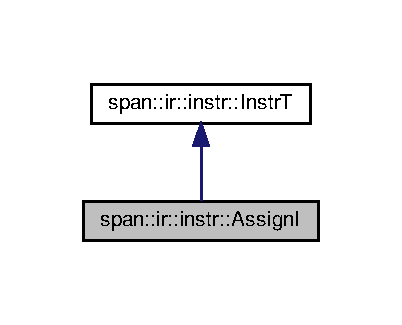
\includegraphics[width=193pt]{classspan_1_1ir_1_1instr_1_1AssignI__inherit__graph}
\end{center}
\end{figure}


Collaboration diagram for span\+:\+:ir\+:\+:instr\+:\+:AssignI\+:\nopagebreak
\begin{figure}[H]
\begin{center}
\leavevmode
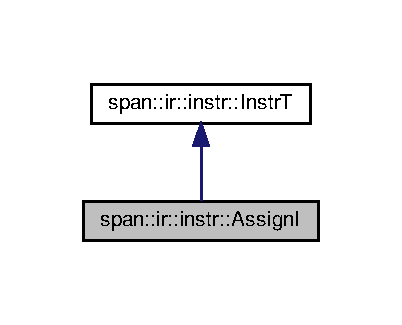
\includegraphics[width=193pt]{classspan_1_1ir_1_1instr_1_1AssignI__coll__graph}
\end{center}
\end{figure}
\subsection*{Public Member Functions}
\begin{DoxyCompactItemize}
\item 
\mbox{\Hypertarget{classspan_1_1ir_1_1instr_1_1AssignI_aa0a0a43086c10e50d1da869cbe4dfe02}\label{classspan_1_1ir_1_1instr_1_1AssignI_aa0a0a43086c10e50d1da869cbe4dfe02}} 
{\bfseries AssignI} (\hyperlink{classspan_1_1ir_1_1expr_1_1VarExpr}{expr\+::\+Var\+Expr} $\ast$lhs, \hyperlink{classspan_1_1ir_1_1expr_1_1Expr}{expr\+::\+Expr} $\ast$rhs)
\item 
\mbox{\Hypertarget{classspan_1_1ir_1_1instr_1_1AssignI_a5c1966b81e7434d6072c104e9ee48a6f}\label{classspan_1_1ir_1_1instr_1_1AssignI_a5c1966b81e7434d6072c104e9ee48a6f}} 
string {\bfseries print} ()
\item 
\mbox{\Hypertarget{classspan_1_1ir_1_1instr_1_1AssignI_a91beb93bf20b53df96ce4872e255d541}\label{classspan_1_1ir_1_1instr_1_1AssignI_a91beb93bf20b53df96ce4872e255d541}} 
{\bfseries AssignI} (\hyperlink{classspan_1_1ir_1_1expr_1_1VarExpr}{expr\+::\+Var\+Expr} $\ast$lhs, \hyperlink{classspan_1_1ir_1_1expr_1_1Expr}{expr\+::\+Expr} $\ast$rhs)
\end{DoxyCompactItemize}


The documentation for this class was generated from the following files\+:\begin{DoxyCompactItemize}
\item 
Instr (copy).\+h\item 
Instr.\+h\item 
Instr.\+cpp\end{DoxyCompactItemize}

\hypertarget{classspan_1_1ir_1_1obj_1_1BB}{}\section{span\+:\+:ir\+:\+:obj\+:\+:BB Class Reference}
\label{classspan_1_1ir_1_1obj_1_1BB}\index{span\+::ir\+::obj\+::\+BB@{span\+::ir\+::obj\+::\+BB}}


A basic block containing a sequence of instructions.  




{\ttfamily \#include $<$objects.\+h$>$}

\subsection*{Private Attributes}
\begin{DoxyCompactItemize}
\item 
\hyperlink{namespacespan_ab988dafbd25ab39838239b91d6a86214}{Basic\+Block\+Id} \hyperlink{classspan_1_1ir_1_1obj_1_1BB_ab0b77a9e575276adaed35fe9ea628e76}{id}
\item 
std\+::vector$<$ InstrT $\ast$ $>$ \hyperlink{classspan_1_1ir_1_1obj_1_1BB_a34eba87f2fb7244ae64b2467c5e7351b}{insns}
\item 
std\+::vector$<$ \hyperlink{classspan_1_1ir_1_1obj_1_1BBEdge}{B\+B\+Edge} $\ast$ $>$ \hyperlink{classspan_1_1ir_1_1obj_1_1BB_a68884bf0898798e8e03477567f231fbb}{in\+Edges}
\item 
std\+::vector$<$ \hyperlink{classspan_1_1ir_1_1obj_1_1BBEdge}{B\+B\+Edge} $\ast$ $>$ \hyperlink{classspan_1_1ir_1_1obj_1_1BB_afc465f9afb8573e400f52fa8641fba85}{out\+Edges}
\item 
std\+::vector$<$ \hyperlink{classspan_1_1ir_1_1obj_1_1CFGNode}{C\+F\+G\+Node} $>$ \hyperlink{classspan_1_1ir_1_1obj_1_1BB_a67209b5148f3bd5cd74657e2d3129e47}{nodes}
\end{DoxyCompactItemize}


\subsection{Detailed Description}
A basic block containing a sequence of instructions. 

\subsection{Member Data Documentation}
\mbox{\Hypertarget{classspan_1_1ir_1_1obj_1_1BB_ab0b77a9e575276adaed35fe9ea628e76}\label{classspan_1_1ir_1_1obj_1_1BB_ab0b77a9e575276adaed35fe9ea628e76}} 
\index{span\+::ir\+::obj\+::\+BB@{span\+::ir\+::obj\+::\+BB}!id@{id}}
\index{id@{id}!span\+::ir\+::obj\+::\+BB@{span\+::ir\+::obj\+::\+BB}}
\subsubsection{\texorpdfstring{id}{id}}
{\footnotesize\ttfamily \hyperlink{namespacespan_ab988dafbd25ab39838239b91d6a86214}{Basic\+Block\+Id} span\+::ir\+::obj\+::\+B\+B\+::id\hspace{0.3cm}{\ttfamily [private]}}

\mbox{\Hypertarget{classspan_1_1ir_1_1obj_1_1BB_a68884bf0898798e8e03477567f231fbb}\label{classspan_1_1ir_1_1obj_1_1BB_a68884bf0898798e8e03477567f231fbb}} 
\index{span\+::ir\+::obj\+::\+BB@{span\+::ir\+::obj\+::\+BB}!in\+Edges@{in\+Edges}}
\index{in\+Edges@{in\+Edges}!span\+::ir\+::obj\+::\+BB@{span\+::ir\+::obj\+::\+BB}}
\subsubsection{\texorpdfstring{in\+Edges}{inEdges}}
{\footnotesize\ttfamily std\+::vector$<$\hyperlink{classspan_1_1ir_1_1obj_1_1BBEdge}{B\+B\+Edge}$\ast$$>$ span\+::ir\+::obj\+::\+B\+B\+::in\+Edges\hspace{0.3cm}{\ttfamily [private]}}

\mbox{\Hypertarget{classspan_1_1ir_1_1obj_1_1BB_a34eba87f2fb7244ae64b2467c5e7351b}\label{classspan_1_1ir_1_1obj_1_1BB_a34eba87f2fb7244ae64b2467c5e7351b}} 
\index{span\+::ir\+::obj\+::\+BB@{span\+::ir\+::obj\+::\+BB}!insns@{insns}}
\index{insns@{insns}!span\+::ir\+::obj\+::\+BB@{span\+::ir\+::obj\+::\+BB}}
\subsubsection{\texorpdfstring{insns}{insns}}
{\footnotesize\ttfamily std\+::vector$<$InstrT$\ast$$>$ span\+::ir\+::obj\+::\+B\+B\+::insns\hspace{0.3cm}{\ttfamily [private]}}

\mbox{\Hypertarget{classspan_1_1ir_1_1obj_1_1BB_a67209b5148f3bd5cd74657e2d3129e47}\label{classspan_1_1ir_1_1obj_1_1BB_a67209b5148f3bd5cd74657e2d3129e47}} 
\index{span\+::ir\+::obj\+::\+BB@{span\+::ir\+::obj\+::\+BB}!nodes@{nodes}}
\index{nodes@{nodes}!span\+::ir\+::obj\+::\+BB@{span\+::ir\+::obj\+::\+BB}}
\subsubsection{\texorpdfstring{nodes}{nodes}}
{\footnotesize\ttfamily std\+::vector$<$\hyperlink{classspan_1_1ir_1_1obj_1_1CFGNode}{C\+F\+G\+Node}$>$ span\+::ir\+::obj\+::\+B\+B\+::nodes\hspace{0.3cm}{\ttfamily [private]}}

\mbox{\Hypertarget{classspan_1_1ir_1_1obj_1_1BB_afc465f9afb8573e400f52fa8641fba85}\label{classspan_1_1ir_1_1obj_1_1BB_afc465f9afb8573e400f52fa8641fba85}} 
\index{span\+::ir\+::obj\+::\+BB@{span\+::ir\+::obj\+::\+BB}!out\+Edges@{out\+Edges}}
\index{out\+Edges@{out\+Edges}!span\+::ir\+::obj\+::\+BB@{span\+::ir\+::obj\+::\+BB}}
\subsubsection{\texorpdfstring{out\+Edges}{outEdges}}
{\footnotesize\ttfamily std\+::vector$<$\hyperlink{classspan_1_1ir_1_1obj_1_1BBEdge}{B\+B\+Edge}$\ast$$>$ span\+::ir\+::obj\+::\+B\+B\+::out\+Edges\hspace{0.3cm}{\ttfamily [private]}}



The documentation for this class was generated from the following file\+:\begin{DoxyCompactItemize}
\item 
\hyperlink{objects_8h}{objects.\+h}\end{DoxyCompactItemize}

\hypertarget{classspan_1_1ir_1_1obj_1_1BBEdge}{}\section{span\+:\+:ir\+:\+:obj\+:\+:B\+B\+Edge Class Reference}
\label{classspan_1_1ir_1_1obj_1_1BBEdge}\index{span\+::ir\+::obj\+::\+B\+B\+Edge@{span\+::ir\+::obj\+::\+B\+B\+Edge}}


A labeled edge connecting basic blocks.  




{\ttfamily \#include $<$objects.\+h$>$}



Collaboration diagram for span\+:\+:ir\+:\+:obj\+:\+:B\+B\+Edge\+:\nopagebreak
\begin{figure}[H]
\begin{center}
\leavevmode
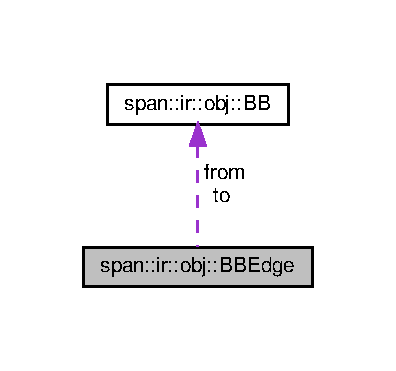
\includegraphics[width=190pt]{classspan_1_1ir_1_1obj_1_1BBEdge__coll__graph}
\end{center}
\end{figure}
\subsection*{Private Attributes}
\begin{DoxyCompactItemize}
\item 
\hyperlink{classspan_1_1ir_1_1obj_1_1BB}{BB} $\ast$ \hyperlink{classspan_1_1ir_1_1obj_1_1BBEdge_a1b9b3319ff37cd051b3a4ec6733656da}{from}
\item 
\hyperlink{classspan_1_1ir_1_1obj_1_1BB}{BB} $\ast$ \hyperlink{classspan_1_1ir_1_1obj_1_1BBEdge_a32bbef719761ee452e6b225551cf3e11}{to}
\item 
\hyperlink{namespacespan_1_1ir_1_1obj_a3687553dc31f18fb1bd62e0798a3f7f0}{Edge\+Kind} \hyperlink{classspan_1_1ir_1_1obj_1_1BBEdge_acf9ddd26f84acad75430f9a19a900440}{edge\+Kind}
\end{DoxyCompactItemize}


\subsection{Detailed Description}
A labeled edge connecting basic blocks. 

\subsection{Member Data Documentation}
\mbox{\Hypertarget{classspan_1_1ir_1_1obj_1_1BBEdge_acf9ddd26f84acad75430f9a19a900440}\label{classspan_1_1ir_1_1obj_1_1BBEdge_acf9ddd26f84acad75430f9a19a900440}} 
\index{span\+::ir\+::obj\+::\+B\+B\+Edge@{span\+::ir\+::obj\+::\+B\+B\+Edge}!edge\+Kind@{edge\+Kind}}
\index{edge\+Kind@{edge\+Kind}!span\+::ir\+::obj\+::\+B\+B\+Edge@{span\+::ir\+::obj\+::\+B\+B\+Edge}}
\subsubsection{\texorpdfstring{edge\+Kind}{edgeKind}}
{\footnotesize\ttfamily \hyperlink{namespacespan_1_1ir_1_1obj_a3687553dc31f18fb1bd62e0798a3f7f0}{Edge\+Kind} span\+::ir\+::obj\+::\+B\+B\+Edge\+::edge\+Kind\hspace{0.3cm}{\ttfamily [private]}}

\mbox{\Hypertarget{classspan_1_1ir_1_1obj_1_1BBEdge_a1b9b3319ff37cd051b3a4ec6733656da}\label{classspan_1_1ir_1_1obj_1_1BBEdge_a1b9b3319ff37cd051b3a4ec6733656da}} 
\index{span\+::ir\+::obj\+::\+B\+B\+Edge@{span\+::ir\+::obj\+::\+B\+B\+Edge}!from@{from}}
\index{from@{from}!span\+::ir\+::obj\+::\+B\+B\+Edge@{span\+::ir\+::obj\+::\+B\+B\+Edge}}
\subsubsection{\texorpdfstring{from}{from}}
{\footnotesize\ttfamily \hyperlink{classspan_1_1ir_1_1obj_1_1BB}{BB}$\ast$ span\+::ir\+::obj\+::\+B\+B\+Edge\+::from\hspace{0.3cm}{\ttfamily [private]}}

\mbox{\Hypertarget{classspan_1_1ir_1_1obj_1_1BBEdge_a32bbef719761ee452e6b225551cf3e11}\label{classspan_1_1ir_1_1obj_1_1BBEdge_a32bbef719761ee452e6b225551cf3e11}} 
\index{span\+::ir\+::obj\+::\+B\+B\+Edge@{span\+::ir\+::obj\+::\+B\+B\+Edge}!to@{to}}
\index{to@{to}!span\+::ir\+::obj\+::\+B\+B\+Edge@{span\+::ir\+::obj\+::\+B\+B\+Edge}}
\subsubsection{\texorpdfstring{to}{to}}
{\footnotesize\ttfamily \hyperlink{classspan_1_1ir_1_1obj_1_1BB}{BB}$\ast$ span\+::ir\+::obj\+::\+B\+B\+Edge\+::to\hspace{0.3cm}{\ttfamily [private]}}



The documentation for this class was generated from the following file\+:\begin{DoxyCompactItemize}
\item 
\hyperlink{objects_8h}{objects.\+h}\end{DoxyCompactItemize}

\hypertarget{classspan_1_1ir_1_1expr_1_1BinaryExpr}{}\section{span\+:\+:ir\+:\+:expr\+:\+:Binary\+Expr Class Reference}
\label{classspan_1_1ir_1_1expr_1_1BinaryExpr}\index{span\+::ir\+::expr\+::\+Binary\+Expr@{span\+::ir\+::expr\+::\+Binary\+Expr}}


{\ttfamily \#include $<$expr.\+h$>$}



Inheritance diagram for span\+:\+:ir\+:\+:expr\+:\+:Binary\+Expr\+:\nopagebreak
\begin{figure}[H]
\begin{center}
\leavevmode
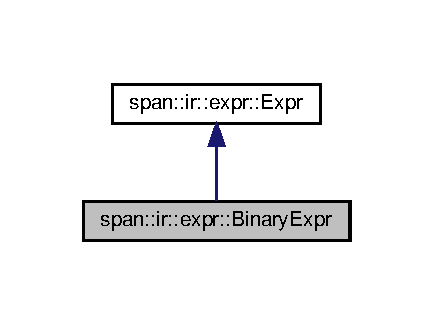
\includegraphics[width=208pt]{classspan_1_1ir_1_1expr_1_1BinaryExpr__inherit__graph}
\end{center}
\end{figure}


Collaboration diagram for span\+:\+:ir\+:\+:expr\+:\+:Binary\+Expr\+:\nopagebreak
\begin{figure}[H]
\begin{center}
\leavevmode
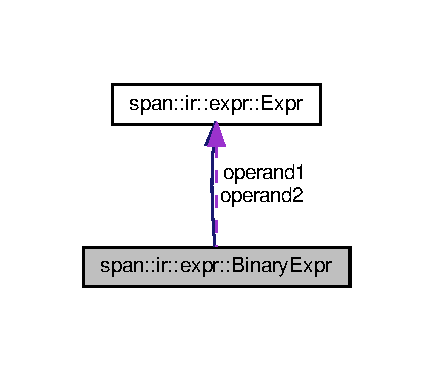
\includegraphics[width=208pt]{classspan_1_1ir_1_1expr_1_1BinaryExpr__coll__graph}
\end{center}
\end{figure}
\subsection*{Private Attributes}
\begin{DoxyCompactItemize}
\item 
Binary\+Operator\+Kind \hyperlink{classspan_1_1ir_1_1expr_1_1BinaryExpr_ab80abc5dcf5f80796c5f720f523f8375}{op\+Code}
\item 
\hyperlink{classspan_1_1ir_1_1expr_1_1Expr}{Expr} $\ast$ \hyperlink{classspan_1_1ir_1_1expr_1_1BinaryExpr_a7aa42a9ab32fe625a6b065601cb5a78f}{operand1}
\item 
\hyperlink{classspan_1_1ir_1_1expr_1_1Expr}{Expr} $\ast$ \hyperlink{classspan_1_1ir_1_1expr_1_1BinaryExpr_a60b088f3fcd2aabbc10445b4c693cfcf}{operand2}
\end{DoxyCompactItemize}


\subsection{Member Data Documentation}
\mbox{\Hypertarget{classspan_1_1ir_1_1expr_1_1BinaryExpr_ab80abc5dcf5f80796c5f720f523f8375}\label{classspan_1_1ir_1_1expr_1_1BinaryExpr_ab80abc5dcf5f80796c5f720f523f8375}} 
\index{span\+::ir\+::expr\+::\+Binary\+Expr@{span\+::ir\+::expr\+::\+Binary\+Expr}!op\+Code@{op\+Code}}
\index{op\+Code@{op\+Code}!span\+::ir\+::expr\+::\+Binary\+Expr@{span\+::ir\+::expr\+::\+Binary\+Expr}}
\subsubsection{\texorpdfstring{op\+Code}{opCode}}
{\footnotesize\ttfamily Binary\+Operator\+Kind span\+::ir\+::expr\+::\+Binary\+Expr\+::op\+Code\hspace{0.3cm}{\ttfamily [private]}}

\mbox{\Hypertarget{classspan_1_1ir_1_1expr_1_1BinaryExpr_a7aa42a9ab32fe625a6b065601cb5a78f}\label{classspan_1_1ir_1_1expr_1_1BinaryExpr_a7aa42a9ab32fe625a6b065601cb5a78f}} 
\index{span\+::ir\+::expr\+::\+Binary\+Expr@{span\+::ir\+::expr\+::\+Binary\+Expr}!operand1@{operand1}}
\index{operand1@{operand1}!span\+::ir\+::expr\+::\+Binary\+Expr@{span\+::ir\+::expr\+::\+Binary\+Expr}}
\subsubsection{\texorpdfstring{operand1}{operand1}}
{\footnotesize\ttfamily \hyperlink{classspan_1_1ir_1_1expr_1_1Expr}{Expr}$\ast$ span\+::ir\+::expr\+::\+Binary\+Expr\+::operand1\hspace{0.3cm}{\ttfamily [private]}}

\mbox{\Hypertarget{classspan_1_1ir_1_1expr_1_1BinaryExpr_a60b088f3fcd2aabbc10445b4c693cfcf}\label{classspan_1_1ir_1_1expr_1_1BinaryExpr_a60b088f3fcd2aabbc10445b4c693cfcf}} 
\index{span\+::ir\+::expr\+::\+Binary\+Expr@{span\+::ir\+::expr\+::\+Binary\+Expr}!operand2@{operand2}}
\index{operand2@{operand2}!span\+::ir\+::expr\+::\+Binary\+Expr@{span\+::ir\+::expr\+::\+Binary\+Expr}}
\subsubsection{\texorpdfstring{operand2}{operand2}}
{\footnotesize\ttfamily \hyperlink{classspan_1_1ir_1_1expr_1_1Expr}{Expr}$\ast$ span\+::ir\+::expr\+::\+Binary\+Expr\+::operand2\hspace{0.3cm}{\ttfamily [private]}}



The documentation for this class was generated from the following file\+:\begin{DoxyCompactItemize}
\item 
\hyperlink{expr_8h}{expr.\+h}\end{DoxyCompactItemize}

\hypertarget{classspan_1_1ir_1_1instr_1_1CallI}{}\section{span\+:\+:ir\+:\+:instr\+:\+:CallI Class Reference}
\label{classspan_1_1ir_1_1instr_1_1CallI}\index{span\+::ir\+::instr\+::\+CallI@{span\+::ir\+::instr\+::\+CallI}}


{\ttfamily \#include $<$instr.\+h$>$}



Inheritance diagram for span\+:\+:ir\+:\+:instr\+:\+:CallI\+:\nopagebreak
\begin{figure}[H]
\begin{center}
\leavevmode
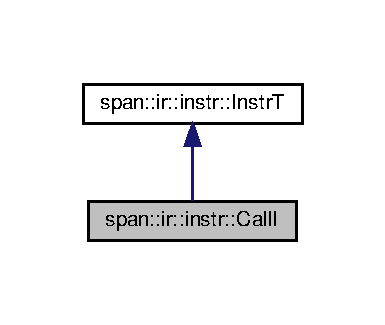
\includegraphics[width=185pt]{classspan_1_1ir_1_1instr_1_1CallI__inherit__graph}
\end{center}
\end{figure}


Collaboration diagram for span\+:\+:ir\+:\+:instr\+:\+:CallI\+:\nopagebreak
\begin{figure}[H]
\begin{center}
\leavevmode
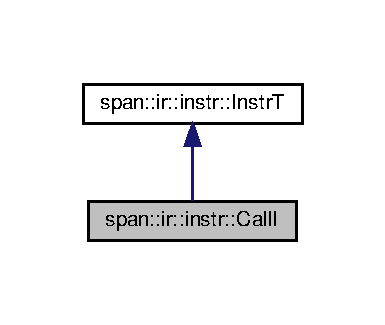
\includegraphics[width=185pt]{classspan_1_1ir_1_1instr_1_1CallI__coll__graph}
\end{center}
\end{figure}


The documentation for this class was generated from the following file\+:\begin{DoxyCompactItemize}
\item 
\hyperlink{instr_8h}{instr.\+h}\end{DoxyCompactItemize}

\hypertarget{classspan_1_1ir_1_1obj_1_1CFG}{}\section{span\+:\+:ir\+:\+:obj\+:\+:C\+FG Class Reference}
\label{classspan_1_1ir_1_1obj_1_1CFG}\index{span\+::ir\+::obj\+::\+C\+FG@{span\+::ir\+::obj\+::\+C\+FG}}


Control Flow Graph.  




{\ttfamily \#include $<$objects.\+h$>$}



Collaboration diagram for span\+:\+:ir\+:\+:obj\+:\+:C\+FG\+:\nopagebreak
\begin{figure}[H]
\begin{center}
\leavevmode
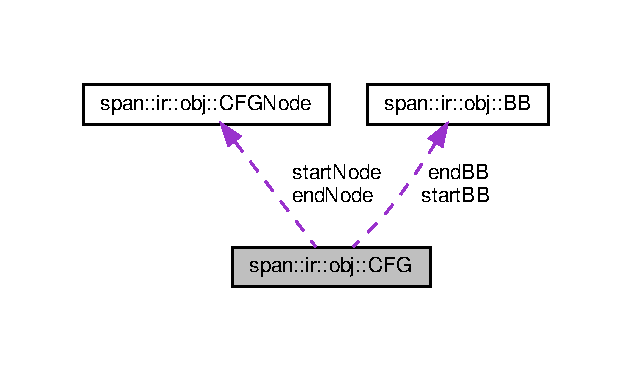
\includegraphics[width=304pt]{classspan_1_1ir_1_1obj_1_1CFG__coll__graph}
\end{center}
\end{figure}
\subsection*{Private Attributes}
\begin{DoxyCompactItemize}
\item 
std\+::unordered\+\_\+map$<$ \hyperlink{namespacespan_ab988dafbd25ab39838239b91d6a86214}{Basic\+Block\+Id}, \hyperlink{classspan_1_1ir_1_1obj_1_1BB}{BB} $>$ \hyperlink{classspan_1_1ir_1_1obj_1_1CFG_ab397d5c00efd9dd6a2ffeb545c16b71b}{bb\+Map}
\item 
std\+::vector$<$ B\+B\+Edge\+Id\+Edge $>$ \hyperlink{classspan_1_1ir_1_1obj_1_1CFG_a2480bf75b73356170ebb4578d4245f33}{bb\+Edges}
\item 
\hyperlink{classspan_1_1ir_1_1obj_1_1BB}{BB} $\ast$ \hyperlink{classspan_1_1ir_1_1obj_1_1CFG_a2a13f446a8367c04a854848ca378d2a3}{start\+BB}
\item 
\hyperlink{classspan_1_1ir_1_1obj_1_1BB}{BB} $\ast$ \hyperlink{classspan_1_1ir_1_1obj_1_1CFG_a7e5b207c46341e1635e9a98bc4b08163}{end\+BB}
\item 
std\+::unordered\+\_\+map$<$ \hyperlink{namespacespan_a34e8d849ca2007fe03cb1817685d08bf}{C\+F\+G\+Node\+Id}, \hyperlink{classspan_1_1ir_1_1obj_1_1CFGNode}{C\+F\+G\+Node} $>$ \hyperlink{classspan_1_1ir_1_1obj_1_1CFG_af11c6fd7a30810fbd49d9162a6b1d5da}{cfg\+Node\+Map}
\item 
std\+::vector$<$ \hyperlink{namespacespan_1_1ir_1_1obj_a8896662ab566cd79d401c0753d3c4120}{C\+F\+G\+Node\+Id\+Edge} $>$ \hyperlink{classspan_1_1ir_1_1obj_1_1CFG_a2352d9b13704a1074df3c8b1553a4c31}{cfg\+Edges}
\item 
\hyperlink{classspan_1_1ir_1_1obj_1_1CFGNode}{C\+F\+G\+Node} $\ast$ \hyperlink{classspan_1_1ir_1_1obj_1_1CFG_a990fe73e4c7c5ea8c6fb563f694787fe}{start\+Node}
\item 
\hyperlink{classspan_1_1ir_1_1obj_1_1CFGNode}{C\+F\+G\+Node} $\ast$ \hyperlink{classspan_1_1ir_1_1obj_1_1CFG_ad6da10e59a29576d2842dbc3ce34cdeb}{end\+Node}
\end{DoxyCompactItemize}


\subsection{Detailed Description}
Control Flow Graph. 

\subsection{Member Data Documentation}
\mbox{\Hypertarget{classspan_1_1ir_1_1obj_1_1CFG_a2480bf75b73356170ebb4578d4245f33}\label{classspan_1_1ir_1_1obj_1_1CFG_a2480bf75b73356170ebb4578d4245f33}} 
\index{span\+::ir\+::obj\+::\+C\+FG@{span\+::ir\+::obj\+::\+C\+FG}!bb\+Edges@{bb\+Edges}}
\index{bb\+Edges@{bb\+Edges}!span\+::ir\+::obj\+::\+C\+FG@{span\+::ir\+::obj\+::\+C\+FG}}
\subsubsection{\texorpdfstring{bb\+Edges}{bbEdges}}
{\footnotesize\ttfamily std\+::vector$<$B\+B\+Edge\+Id\+Edge$>$ span\+::ir\+::obj\+::\+C\+F\+G\+::bb\+Edges\hspace{0.3cm}{\ttfamily [private]}}

\mbox{\Hypertarget{classspan_1_1ir_1_1obj_1_1CFG_ab397d5c00efd9dd6a2ffeb545c16b71b}\label{classspan_1_1ir_1_1obj_1_1CFG_ab397d5c00efd9dd6a2ffeb545c16b71b}} 
\index{span\+::ir\+::obj\+::\+C\+FG@{span\+::ir\+::obj\+::\+C\+FG}!bb\+Map@{bb\+Map}}
\index{bb\+Map@{bb\+Map}!span\+::ir\+::obj\+::\+C\+FG@{span\+::ir\+::obj\+::\+C\+FG}}
\subsubsection{\texorpdfstring{bb\+Map}{bbMap}}
{\footnotesize\ttfamily std\+::unordered\+\_\+map$<$\hyperlink{namespacespan_ab988dafbd25ab39838239b91d6a86214}{Basic\+Block\+Id}, \hyperlink{classspan_1_1ir_1_1obj_1_1BB}{BB}$>$ span\+::ir\+::obj\+::\+C\+F\+G\+::bb\+Map\hspace{0.3cm}{\ttfamily [private]}}

\mbox{\Hypertarget{classspan_1_1ir_1_1obj_1_1CFG_a2352d9b13704a1074df3c8b1553a4c31}\label{classspan_1_1ir_1_1obj_1_1CFG_a2352d9b13704a1074df3c8b1553a4c31}} 
\index{span\+::ir\+::obj\+::\+C\+FG@{span\+::ir\+::obj\+::\+C\+FG}!cfg\+Edges@{cfg\+Edges}}
\index{cfg\+Edges@{cfg\+Edges}!span\+::ir\+::obj\+::\+C\+FG@{span\+::ir\+::obj\+::\+C\+FG}}
\subsubsection{\texorpdfstring{cfg\+Edges}{cfgEdges}}
{\footnotesize\ttfamily std\+::vector$<$\hyperlink{namespacespan_1_1ir_1_1obj_a8896662ab566cd79d401c0753d3c4120}{C\+F\+G\+Node\+Id\+Edge}$>$ span\+::ir\+::obj\+::\+C\+F\+G\+::cfg\+Edges\hspace{0.3cm}{\ttfamily [private]}}

\mbox{\Hypertarget{classspan_1_1ir_1_1obj_1_1CFG_af11c6fd7a30810fbd49d9162a6b1d5da}\label{classspan_1_1ir_1_1obj_1_1CFG_af11c6fd7a30810fbd49d9162a6b1d5da}} 
\index{span\+::ir\+::obj\+::\+C\+FG@{span\+::ir\+::obj\+::\+C\+FG}!cfg\+Node\+Map@{cfg\+Node\+Map}}
\index{cfg\+Node\+Map@{cfg\+Node\+Map}!span\+::ir\+::obj\+::\+C\+FG@{span\+::ir\+::obj\+::\+C\+FG}}
\subsubsection{\texorpdfstring{cfg\+Node\+Map}{cfgNodeMap}}
{\footnotesize\ttfamily std\+::unordered\+\_\+map$<$\hyperlink{namespacespan_a34e8d849ca2007fe03cb1817685d08bf}{C\+F\+G\+Node\+Id}, \hyperlink{classspan_1_1ir_1_1obj_1_1CFGNode}{C\+F\+G\+Node}$>$ span\+::ir\+::obj\+::\+C\+F\+G\+::cfg\+Node\+Map\hspace{0.3cm}{\ttfamily [private]}}

\mbox{\Hypertarget{classspan_1_1ir_1_1obj_1_1CFG_a7e5b207c46341e1635e9a98bc4b08163}\label{classspan_1_1ir_1_1obj_1_1CFG_a7e5b207c46341e1635e9a98bc4b08163}} 
\index{span\+::ir\+::obj\+::\+C\+FG@{span\+::ir\+::obj\+::\+C\+FG}!end\+BB@{end\+BB}}
\index{end\+BB@{end\+BB}!span\+::ir\+::obj\+::\+C\+FG@{span\+::ir\+::obj\+::\+C\+FG}}
\subsubsection{\texorpdfstring{end\+BB}{endBB}}
{\footnotesize\ttfamily \hyperlink{classspan_1_1ir_1_1obj_1_1BB}{BB}$\ast$ span\+::ir\+::obj\+::\+C\+F\+G\+::end\+BB\hspace{0.3cm}{\ttfamily [private]}}

\mbox{\Hypertarget{classspan_1_1ir_1_1obj_1_1CFG_ad6da10e59a29576d2842dbc3ce34cdeb}\label{classspan_1_1ir_1_1obj_1_1CFG_ad6da10e59a29576d2842dbc3ce34cdeb}} 
\index{span\+::ir\+::obj\+::\+C\+FG@{span\+::ir\+::obj\+::\+C\+FG}!end\+Node@{end\+Node}}
\index{end\+Node@{end\+Node}!span\+::ir\+::obj\+::\+C\+FG@{span\+::ir\+::obj\+::\+C\+FG}}
\subsubsection{\texorpdfstring{end\+Node}{endNode}}
{\footnotesize\ttfamily \hyperlink{classspan_1_1ir_1_1obj_1_1CFGNode}{C\+F\+G\+Node}$\ast$ span\+::ir\+::obj\+::\+C\+F\+G\+::end\+Node\hspace{0.3cm}{\ttfamily [private]}}

\mbox{\Hypertarget{classspan_1_1ir_1_1obj_1_1CFG_a2a13f446a8367c04a854848ca378d2a3}\label{classspan_1_1ir_1_1obj_1_1CFG_a2a13f446a8367c04a854848ca378d2a3}} 
\index{span\+::ir\+::obj\+::\+C\+FG@{span\+::ir\+::obj\+::\+C\+FG}!start\+BB@{start\+BB}}
\index{start\+BB@{start\+BB}!span\+::ir\+::obj\+::\+C\+FG@{span\+::ir\+::obj\+::\+C\+FG}}
\subsubsection{\texorpdfstring{start\+BB}{startBB}}
{\footnotesize\ttfamily \hyperlink{classspan_1_1ir_1_1obj_1_1BB}{BB}$\ast$ span\+::ir\+::obj\+::\+C\+F\+G\+::start\+BB\hspace{0.3cm}{\ttfamily [private]}}

\mbox{\Hypertarget{classspan_1_1ir_1_1obj_1_1CFG_a990fe73e4c7c5ea8c6fb563f694787fe}\label{classspan_1_1ir_1_1obj_1_1CFG_a990fe73e4c7c5ea8c6fb563f694787fe}} 
\index{span\+::ir\+::obj\+::\+C\+FG@{span\+::ir\+::obj\+::\+C\+FG}!start\+Node@{start\+Node}}
\index{start\+Node@{start\+Node}!span\+::ir\+::obj\+::\+C\+FG@{span\+::ir\+::obj\+::\+C\+FG}}
\subsubsection{\texorpdfstring{start\+Node}{startNode}}
{\footnotesize\ttfamily \hyperlink{classspan_1_1ir_1_1obj_1_1CFGNode}{C\+F\+G\+Node}$\ast$ span\+::ir\+::obj\+::\+C\+F\+G\+::start\+Node\hspace{0.3cm}{\ttfamily [private]}}



The documentation for this class was generated from the following file\+:\begin{DoxyCompactItemize}
\item 
\hyperlink{objects_8h}{objects.\+h}\end{DoxyCompactItemize}

\hypertarget{classspan_1_1ir_1_1obj_1_1CFGNode}{}\section{span\+:\+:ir\+:\+:obj\+:\+:C\+F\+G\+Node Class Reference}
\label{classspan_1_1ir_1_1obj_1_1CFGNode}\index{span\+::ir\+::obj\+::\+C\+F\+G\+Node@{span\+::ir\+::obj\+::\+C\+F\+G\+Node}}


A \hyperlink{classspan_1_1ir_1_1obj_1_1CFG}{C\+FG} Node.  




{\ttfamily \#include $<$objects.\+h$>$}

\subsection*{Private Attributes}
\begin{DoxyCompactItemize}
\item 
InstrT $\ast$ \hyperlink{classspan_1_1ir_1_1obj_1_1CFGNode_a9b5037f569e7e6bcd38117009134a03b}{insn}
\item 
std\+::vector$<$ \hyperlink{classspan_1_1ir_1_1obj_1_1CFGNodeEdge}{C\+F\+G\+Node\+Edge} $\ast$ $>$ \hyperlink{classspan_1_1ir_1_1obj_1_1CFGNode_a8c47bc484535d940978469b85447b812}{in\+Edges}
\item 
std\+::vector$<$ \hyperlink{classspan_1_1ir_1_1obj_1_1CFGNodeEdge}{C\+F\+G\+Node\+Edge} $\ast$ $>$ \hyperlink{classspan_1_1ir_1_1obj_1_1CFGNode_afd6aa8d1ec4f152e752290d7f5c52dba}{out\+Edges}
\end{DoxyCompactItemize}


\subsection{Detailed Description}
A \hyperlink{classspan_1_1ir_1_1obj_1_1CFG}{C\+FG} Node. 

\subsection{Member Data Documentation}
\mbox{\Hypertarget{classspan_1_1ir_1_1obj_1_1CFGNode_a8c47bc484535d940978469b85447b812}\label{classspan_1_1ir_1_1obj_1_1CFGNode_a8c47bc484535d940978469b85447b812}} 
\index{span\+::ir\+::obj\+::\+C\+F\+G\+Node@{span\+::ir\+::obj\+::\+C\+F\+G\+Node}!in\+Edges@{in\+Edges}}
\index{in\+Edges@{in\+Edges}!span\+::ir\+::obj\+::\+C\+F\+G\+Node@{span\+::ir\+::obj\+::\+C\+F\+G\+Node}}
\subsubsection{\texorpdfstring{in\+Edges}{inEdges}}
{\footnotesize\ttfamily std\+::vector$<$\hyperlink{classspan_1_1ir_1_1obj_1_1CFGNodeEdge}{C\+F\+G\+Node\+Edge}$\ast$$>$ span\+::ir\+::obj\+::\+C\+F\+G\+Node\+::in\+Edges\hspace{0.3cm}{\ttfamily [private]}}

\mbox{\Hypertarget{classspan_1_1ir_1_1obj_1_1CFGNode_a9b5037f569e7e6bcd38117009134a03b}\label{classspan_1_1ir_1_1obj_1_1CFGNode_a9b5037f569e7e6bcd38117009134a03b}} 
\index{span\+::ir\+::obj\+::\+C\+F\+G\+Node@{span\+::ir\+::obj\+::\+C\+F\+G\+Node}!insn@{insn}}
\index{insn@{insn}!span\+::ir\+::obj\+::\+C\+F\+G\+Node@{span\+::ir\+::obj\+::\+C\+F\+G\+Node}}
\subsubsection{\texorpdfstring{insn}{insn}}
{\footnotesize\ttfamily InstrT$\ast$ span\+::ir\+::obj\+::\+C\+F\+G\+Node\+::insn\hspace{0.3cm}{\ttfamily [private]}}

\mbox{\Hypertarget{classspan_1_1ir_1_1obj_1_1CFGNode_afd6aa8d1ec4f152e752290d7f5c52dba}\label{classspan_1_1ir_1_1obj_1_1CFGNode_afd6aa8d1ec4f152e752290d7f5c52dba}} 
\index{span\+::ir\+::obj\+::\+C\+F\+G\+Node@{span\+::ir\+::obj\+::\+C\+F\+G\+Node}!out\+Edges@{out\+Edges}}
\index{out\+Edges@{out\+Edges}!span\+::ir\+::obj\+::\+C\+F\+G\+Node@{span\+::ir\+::obj\+::\+C\+F\+G\+Node}}
\subsubsection{\texorpdfstring{out\+Edges}{outEdges}}
{\footnotesize\ttfamily std\+::vector$<$\hyperlink{classspan_1_1ir_1_1obj_1_1CFGNodeEdge}{C\+F\+G\+Node\+Edge}$\ast$$>$ span\+::ir\+::obj\+::\+C\+F\+G\+Node\+::out\+Edges\hspace{0.3cm}{\ttfamily [private]}}



The documentation for this class was generated from the following file\+:\begin{DoxyCompactItemize}
\item 
\hyperlink{objects_8h}{objects.\+h}\end{DoxyCompactItemize}

\hypertarget{classspan_1_1ir_1_1obj_1_1CFGNodeEdge}{}\section{span\+:\+:ir\+:\+:obj\+:\+:C\+F\+G\+Node\+Edge Class Reference}
\label{classspan_1_1ir_1_1obj_1_1CFGNodeEdge}\index{span\+::ir\+::obj\+::\+C\+F\+G\+Node\+Edge@{span\+::ir\+::obj\+::\+C\+F\+G\+Node\+Edge}}


A labeled edge connecting \hyperlink{classspan_1_1ir_1_1obj_1_1CFG}{C\+FG} Nodes.  




{\ttfamily \#include $<$objects.\+h$>$}



Collaboration diagram for span\+:\+:ir\+:\+:obj\+:\+:C\+F\+G\+Node\+Edge\+:\nopagebreak
\begin{figure}[H]
\begin{center}
\leavevmode
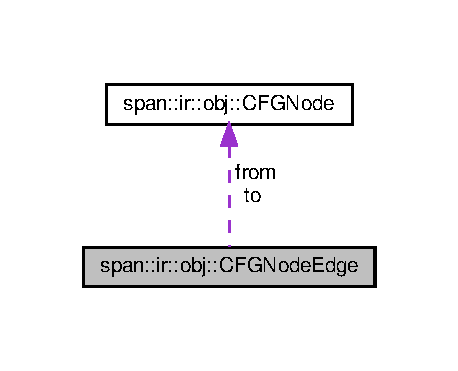
\includegraphics[width=220pt]{classspan_1_1ir_1_1obj_1_1CFGNodeEdge__coll__graph}
\end{center}
\end{figure}
\subsection*{Private Attributes}
\begin{DoxyCompactItemize}
\item 
\hyperlink{classspan_1_1ir_1_1obj_1_1CFGNode}{C\+F\+G\+Node} $\ast$ \hyperlink{classspan_1_1ir_1_1obj_1_1CFGNodeEdge_a1073fbe480fa96cba7f0aada4edd5c86}{from}
\item 
\hyperlink{classspan_1_1ir_1_1obj_1_1CFGNode}{C\+F\+G\+Node} $\ast$ \hyperlink{classspan_1_1ir_1_1obj_1_1CFGNodeEdge_a4ab4504dcafd1b370e7cc471ecc734db}{to}
\item 
\hyperlink{namespacespan_1_1ir_1_1obj_a3687553dc31f18fb1bd62e0798a3f7f0}{Edge\+Kind} \hyperlink{classspan_1_1ir_1_1obj_1_1CFGNodeEdge_a92bdcf866da2ef6d9836840f2e69a202}{edge\+Kind}
\end{DoxyCompactItemize}


\subsection{Detailed Description}
A labeled edge connecting \hyperlink{classspan_1_1ir_1_1obj_1_1CFG}{C\+FG} Nodes. 

\subsection{Member Data Documentation}
\mbox{\Hypertarget{classspan_1_1ir_1_1obj_1_1CFGNodeEdge_a92bdcf866da2ef6d9836840f2e69a202}\label{classspan_1_1ir_1_1obj_1_1CFGNodeEdge_a92bdcf866da2ef6d9836840f2e69a202}} 
\index{span\+::ir\+::obj\+::\+C\+F\+G\+Node\+Edge@{span\+::ir\+::obj\+::\+C\+F\+G\+Node\+Edge}!edge\+Kind@{edge\+Kind}}
\index{edge\+Kind@{edge\+Kind}!span\+::ir\+::obj\+::\+C\+F\+G\+Node\+Edge@{span\+::ir\+::obj\+::\+C\+F\+G\+Node\+Edge}}
\subsubsection{\texorpdfstring{edge\+Kind}{edgeKind}}
{\footnotesize\ttfamily \hyperlink{namespacespan_1_1ir_1_1obj_a3687553dc31f18fb1bd62e0798a3f7f0}{Edge\+Kind} span\+::ir\+::obj\+::\+C\+F\+G\+Node\+Edge\+::edge\+Kind\hspace{0.3cm}{\ttfamily [private]}}

\mbox{\Hypertarget{classspan_1_1ir_1_1obj_1_1CFGNodeEdge_a1073fbe480fa96cba7f0aada4edd5c86}\label{classspan_1_1ir_1_1obj_1_1CFGNodeEdge_a1073fbe480fa96cba7f0aada4edd5c86}} 
\index{span\+::ir\+::obj\+::\+C\+F\+G\+Node\+Edge@{span\+::ir\+::obj\+::\+C\+F\+G\+Node\+Edge}!from@{from}}
\index{from@{from}!span\+::ir\+::obj\+::\+C\+F\+G\+Node\+Edge@{span\+::ir\+::obj\+::\+C\+F\+G\+Node\+Edge}}
\subsubsection{\texorpdfstring{from}{from}}
{\footnotesize\ttfamily \hyperlink{classspan_1_1ir_1_1obj_1_1CFGNode}{C\+F\+G\+Node}$\ast$ span\+::ir\+::obj\+::\+C\+F\+G\+Node\+Edge\+::from\hspace{0.3cm}{\ttfamily [private]}}

\mbox{\Hypertarget{classspan_1_1ir_1_1obj_1_1CFGNodeEdge_a4ab4504dcafd1b370e7cc471ecc734db}\label{classspan_1_1ir_1_1obj_1_1CFGNodeEdge_a4ab4504dcafd1b370e7cc471ecc734db}} 
\index{span\+::ir\+::obj\+::\+C\+F\+G\+Node\+Edge@{span\+::ir\+::obj\+::\+C\+F\+G\+Node\+Edge}!to@{to}}
\index{to@{to}!span\+::ir\+::obj\+::\+C\+F\+G\+Node\+Edge@{span\+::ir\+::obj\+::\+C\+F\+G\+Node\+Edge}}
\subsubsection{\texorpdfstring{to}{to}}
{\footnotesize\ttfamily \hyperlink{classspan_1_1ir_1_1obj_1_1CFGNode}{C\+F\+G\+Node}$\ast$ span\+::ir\+::obj\+::\+C\+F\+G\+Node\+Edge\+::to\hspace{0.3cm}{\ttfamily [private]}}



The documentation for this class was generated from the following file\+:\begin{DoxyCompactItemize}
\item 
\hyperlink{objects_8h}{objects.\+h}\end{DoxyCompactItemize}

\hypertarget{classspan_1_1ir_1_1expr_1_1Expr}{}\section{span\+:\+:ir\+:\+:expr\+:\+:Expr Class Reference}
\label{classspan_1_1ir_1_1expr_1_1Expr}\index{span\+::ir\+::expr\+::\+Expr@{span\+::ir\+::expr\+::\+Expr}}


Inheritance diagram for span\+:\+:ir\+:\+:expr\+:\+:Expr\+:\nopagebreak
\begin{figure}[H]
\begin{center}
\leavevmode
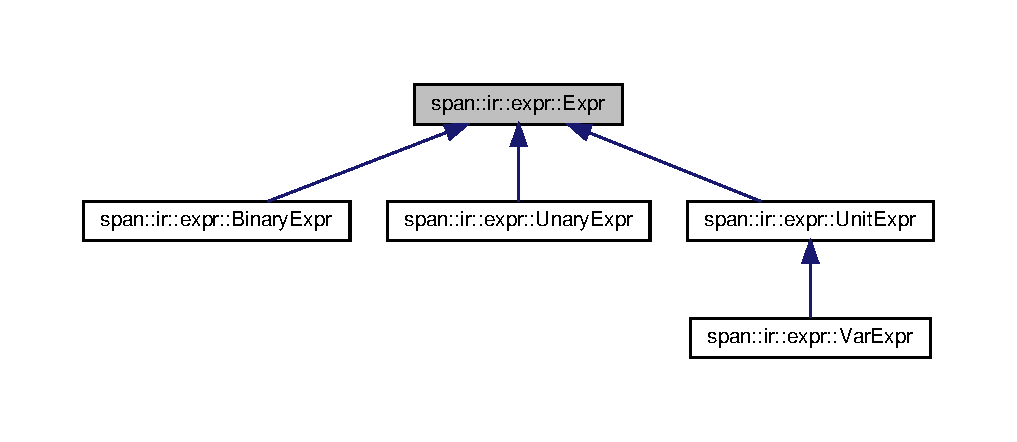
\includegraphics[width=350pt]{classspan_1_1ir_1_1expr_1_1Expr__inherit__graph}
\end{center}
\end{figure}
\subsection*{Public Member Functions}
\begin{DoxyCompactItemize}
\item 
\mbox{\Hypertarget{classspan_1_1ir_1_1expr_1_1Expr_a0993178d09f21dc6afd8f381db2ef109}\label{classspan_1_1ir_1_1expr_1_1Expr_a0993178d09f21dc6afd8f381db2ef109}} 
{\bfseries Expr} (\hyperlink{classspan_1_1ir_1_1types_1_1Type}{types\+::\+Type} $\ast$type, Basic\+Expr\+Kinds expr\+Code)
\item 
\mbox{\Hypertarget{classspan_1_1ir_1_1expr_1_1Expr_adaa50ac1b56440f2c2210027793f304d}\label{classspan_1_1ir_1_1expr_1_1Expr_adaa50ac1b56440f2c2210027793f304d}} 
string {\bfseries print} ()
\item 
\mbox{\Hypertarget{classspan_1_1ir_1_1expr_1_1Expr_a498699f7d37feb602056dcc76bc5f3e2}\label{classspan_1_1ir_1_1expr_1_1Expr_a498699f7d37feb602056dcc76bc5f3e2}} 
\hyperlink{classspan_1_1ir_1_1types_1_1Type}{types\+::\+Type} $\ast$ {\bfseries get\+Type} ()
\item 
\mbox{\Hypertarget{classspan_1_1ir_1_1expr_1_1Expr_a060597873ffabf72a7827149a8d997b1}\label{classspan_1_1ir_1_1expr_1_1Expr_a060597873ffabf72a7827149a8d997b1}} 
types\+::\+Basic\+Type\+Kinds {\bfseries get\+Type\+Code} ()
\item 
\mbox{\Hypertarget{classspan_1_1ir_1_1expr_1_1Expr_af8beed4c9324873f227c177ce71b12b0}\label{classspan_1_1ir_1_1expr_1_1Expr_af8beed4c9324873f227c177ce71b12b0}} 
{\bfseries Expr} (\hyperlink{classspan_1_1ir_1_1types_1_1Type}{types\+::\+Type} $\ast$type, Basic\+Expr\+Kinds expr\+Code)
\item 
\mbox{\Hypertarget{classspan_1_1ir_1_1expr_1_1Expr_a2f17543c09e42dfdb354b58d0a05877b}\label{classspan_1_1ir_1_1expr_1_1Expr_a2f17543c09e42dfdb354b58d0a05877b}} 
void {\bfseries print} ()
\item 
\mbox{\Hypertarget{classspan_1_1ir_1_1expr_1_1Expr_a5d21a4fa7eaefbf7d9804f307310e588}\label{classspan_1_1ir_1_1expr_1_1Expr_a5d21a4fa7eaefbf7d9804f307310e588}} 
\hyperlink{classspan_1_1ir_1_1types_1_1Type}{types\+::\+Type} $\ast$ {\bfseries get\+Type} ()
\item 
\mbox{\Hypertarget{classspan_1_1ir_1_1expr_1_1Expr_a981199f2ab1c4cae88252b1db285cce2}\label{classspan_1_1ir_1_1expr_1_1Expr_a981199f2ab1c4cae88252b1db285cce2}} 
types\+::\+Basic\+Type\+Kinds {\bfseries get\+Type\+Code} ()
\end{DoxyCompactItemize}


The documentation for this class was generated from the following files\+:\begin{DoxyCompactItemize}
\item 
Expr (copy).\+h\item 
Expr.\+h\item 
Expr.\+cpp\end{DoxyCompactItemize}

\hypertarget{classspan_1_1ir_1_1types_1_1Function}{}\section{span\+:\+:ir\+:\+:types\+:\+:Function Class Reference}
\label{classspan_1_1ir_1_1types_1_1Function}\index{span\+::ir\+::types\+::\+Function@{span\+::ir\+::types\+::\+Function}}


{\ttfamily \#include $<$types.\+h$>$}



Inheritance diagram for span\+:\+:ir\+:\+:types\+:\+:Function\+:\nopagebreak
\begin{figure}[H]
\begin{center}
\leavevmode
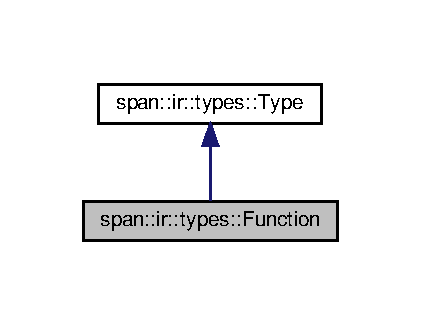
\includegraphics[width=202pt]{classspan_1_1ir_1_1types_1_1Function__inherit__graph}
\end{center}
\end{figure}


Collaboration diagram for span\+:\+:ir\+:\+:types\+:\+:Function\+:\nopagebreak
\begin{figure}[H]
\begin{center}
\leavevmode
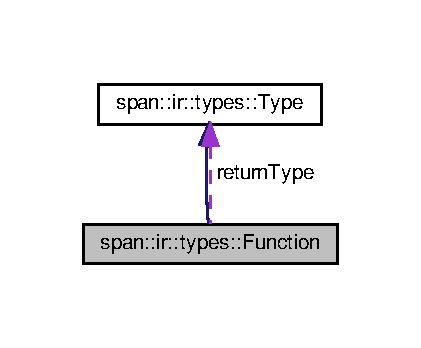
\includegraphics[width=202pt]{classspan_1_1ir_1_1types_1_1Function__coll__graph}
\end{center}
\end{figure}
\subsection*{Private Attributes}
\begin{DoxyCompactItemize}
\item 
\hyperlink{classspan_1_1ir_1_1types_1_1Type}{Type} $\ast$ \hyperlink{classspan_1_1ir_1_1types_1_1Function_a15ff7705df3fde0945e5af56860427fd}{return\+Type}
\item 
std\+::vector$<$ \hyperlink{classspan_1_1ir_1_1types_1_1Type}{Type} $\ast$ $>$ \hyperlink{classspan_1_1ir_1_1types_1_1Function_a8d4a9b7c9cbbfead9d1c7c44bef9bbfd}{params}
\item 
bool \hyperlink{classspan_1_1ir_1_1types_1_1Function_a80c12a5f75fe5c1db469bb0a202987d6}{variadic}
\end{DoxyCompactItemize}
\subsection*{Additional Inherited Members}


\subsection{Member Data Documentation}
\mbox{\Hypertarget{classspan_1_1ir_1_1types_1_1Function_a8d4a9b7c9cbbfead9d1c7c44bef9bbfd}\label{classspan_1_1ir_1_1types_1_1Function_a8d4a9b7c9cbbfead9d1c7c44bef9bbfd}} 
\index{span\+::ir\+::types\+::\+Function@{span\+::ir\+::types\+::\+Function}!params@{params}}
\index{params@{params}!span\+::ir\+::types\+::\+Function@{span\+::ir\+::types\+::\+Function}}
\subsubsection{\texorpdfstring{params}{params}}
{\footnotesize\ttfamily std\+::vector$<$\hyperlink{classspan_1_1ir_1_1types_1_1Type}{Type}$\ast$$>$ span\+::ir\+::types\+::\+Function\+::params\hspace{0.3cm}{\ttfamily [private]}}

\mbox{\Hypertarget{classspan_1_1ir_1_1types_1_1Function_a15ff7705df3fde0945e5af56860427fd}\label{classspan_1_1ir_1_1types_1_1Function_a15ff7705df3fde0945e5af56860427fd}} 
\index{span\+::ir\+::types\+::\+Function@{span\+::ir\+::types\+::\+Function}!return\+Type@{return\+Type}}
\index{return\+Type@{return\+Type}!span\+::ir\+::types\+::\+Function@{span\+::ir\+::types\+::\+Function}}
\subsubsection{\texorpdfstring{return\+Type}{returnType}}
{\footnotesize\ttfamily \hyperlink{classspan_1_1ir_1_1types_1_1Type}{Type}$\ast$ span\+::ir\+::types\+::\+Function\+::return\+Type\hspace{0.3cm}{\ttfamily [private]}}

\mbox{\Hypertarget{classspan_1_1ir_1_1types_1_1Function_a80c12a5f75fe5c1db469bb0a202987d6}\label{classspan_1_1ir_1_1types_1_1Function_a80c12a5f75fe5c1db469bb0a202987d6}} 
\index{span\+::ir\+::types\+::\+Function@{span\+::ir\+::types\+::\+Function}!variadic@{variadic}}
\index{variadic@{variadic}!span\+::ir\+::types\+::\+Function@{span\+::ir\+::types\+::\+Function}}
\subsubsection{\texorpdfstring{variadic}{variadic}}
{\footnotesize\ttfamily bool span\+::ir\+::types\+::\+Function\+::variadic\hspace{0.3cm}{\ttfamily [private]}}



The documentation for this class was generated from the following file\+:\begin{DoxyCompactItemize}
\item 
\hyperlink{types_8h}{types.\+h}\end{DoxyCompactItemize}

\hypertarget{classspan_1_1ir_1_1obj_1_1Function}{}\section{span\+:\+:ir\+:\+:obj\+:\+:Function Class Reference}
\label{classspan_1_1ir_1_1obj_1_1Function}\index{span\+::ir\+::obj\+::\+Function@{span\+::ir\+::obj\+::\+Function}}


A function declaration/definition.  




{\ttfamily \#include $<$objects.\+h$>$}



Collaboration diagram for span\+:\+:ir\+:\+:obj\+:\+:Function\+:\nopagebreak
\begin{figure}[H]
\begin{center}
\leavevmode
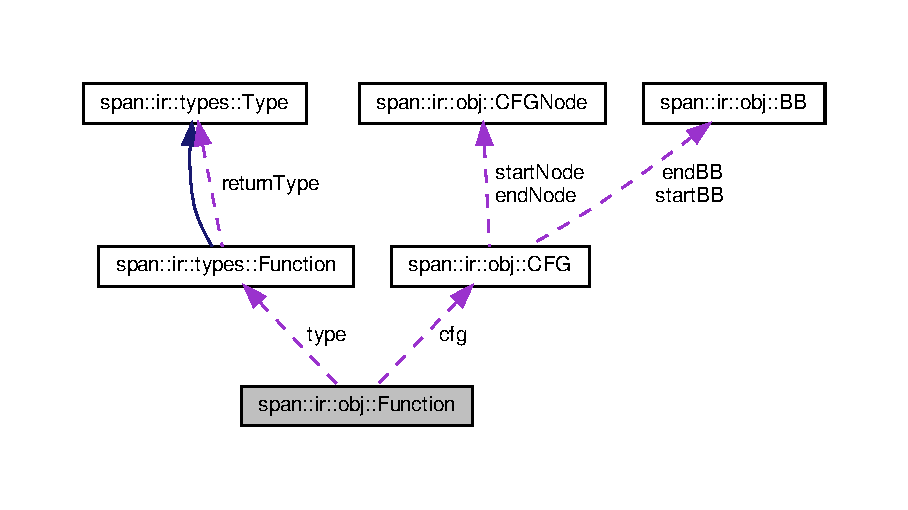
\includegraphics[width=350pt]{classspan_1_1ir_1_1obj_1_1Function__coll__graph}
\end{center}
\end{figure}
\subsection*{Private Attributes}
\begin{DoxyCompactItemize}
\item 
std\+::string \hyperlink{classspan_1_1ir_1_1obj_1_1Function_afb7dc1b55c81492a1243b75734add6ab}{name}
\item 
\hyperlink{classspan_1_1ir_1_1types_1_1Function}{types\+::\+Function} \hyperlink{classspan_1_1ir_1_1obj_1_1Function_af2916d791297d39a30c4c597b73d38b3}{type}
\item 
std\+::vector$<$ std\+::string $>$ \hyperlink{classspan_1_1ir_1_1obj_1_1Function_a1716aaabf39b86d19258a87cde9ba344}{param\+Names}
\item 
std\+::vector$<$ \hyperlink{classspan_1_1ir_1_1instr_1_1InstrT}{instr\+::\+InstrT} $\ast$ $>$ \hyperlink{classspan_1_1ir_1_1obj_1_1Function_a67f2ae04de111d711a08291b7621e6fd}{insns}
\item 
\hyperlink{classspan_1_1ir_1_1obj_1_1CFG}{C\+FG} \hyperlink{classspan_1_1ir_1_1obj_1_1Function_a992bc96ffb731851bc6773fbb11f4095}{cfg}
\item 
bool \hyperlink{classspan_1_1ir_1_1obj_1_1Function_a5c761b10e89a5b9a22804728c2bba800}{body}
\end{DoxyCompactItemize}


\subsection{Detailed Description}
A function declaration/definition. 

\subsection{Member Data Documentation}
\mbox{\Hypertarget{classspan_1_1ir_1_1obj_1_1Function_a5c761b10e89a5b9a22804728c2bba800}\label{classspan_1_1ir_1_1obj_1_1Function_a5c761b10e89a5b9a22804728c2bba800}} 
\index{span\+::ir\+::obj\+::\+Function@{span\+::ir\+::obj\+::\+Function}!body@{body}}
\index{body@{body}!span\+::ir\+::obj\+::\+Function@{span\+::ir\+::obj\+::\+Function}}
\subsubsection{\texorpdfstring{body}{body}}
{\footnotesize\ttfamily bool span\+::ir\+::obj\+::\+Function\+::body\hspace{0.3cm}{\ttfamily [private]}}

\mbox{\Hypertarget{classspan_1_1ir_1_1obj_1_1Function_a992bc96ffb731851bc6773fbb11f4095}\label{classspan_1_1ir_1_1obj_1_1Function_a992bc96ffb731851bc6773fbb11f4095}} 
\index{span\+::ir\+::obj\+::\+Function@{span\+::ir\+::obj\+::\+Function}!cfg@{cfg}}
\index{cfg@{cfg}!span\+::ir\+::obj\+::\+Function@{span\+::ir\+::obj\+::\+Function}}
\subsubsection{\texorpdfstring{cfg}{cfg}}
{\footnotesize\ttfamily \hyperlink{classspan_1_1ir_1_1obj_1_1CFG}{C\+FG} span\+::ir\+::obj\+::\+Function\+::cfg\hspace{0.3cm}{\ttfamily [private]}}

\mbox{\Hypertarget{classspan_1_1ir_1_1obj_1_1Function_a67f2ae04de111d711a08291b7621e6fd}\label{classspan_1_1ir_1_1obj_1_1Function_a67f2ae04de111d711a08291b7621e6fd}} 
\index{span\+::ir\+::obj\+::\+Function@{span\+::ir\+::obj\+::\+Function}!insns@{insns}}
\index{insns@{insns}!span\+::ir\+::obj\+::\+Function@{span\+::ir\+::obj\+::\+Function}}
\subsubsection{\texorpdfstring{insns}{insns}}
{\footnotesize\ttfamily std\+::vector$<$\hyperlink{classspan_1_1ir_1_1instr_1_1InstrT}{instr\+::\+InstrT}$\ast$$>$ span\+::ir\+::obj\+::\+Function\+::insns\hspace{0.3cm}{\ttfamily [private]}}

\mbox{\Hypertarget{classspan_1_1ir_1_1obj_1_1Function_afb7dc1b55c81492a1243b75734add6ab}\label{classspan_1_1ir_1_1obj_1_1Function_afb7dc1b55c81492a1243b75734add6ab}} 
\index{span\+::ir\+::obj\+::\+Function@{span\+::ir\+::obj\+::\+Function}!name@{name}}
\index{name@{name}!span\+::ir\+::obj\+::\+Function@{span\+::ir\+::obj\+::\+Function}}
\subsubsection{\texorpdfstring{name}{name}}
{\footnotesize\ttfamily std\+::string span\+::ir\+::obj\+::\+Function\+::name\hspace{0.3cm}{\ttfamily [private]}}

\mbox{\Hypertarget{classspan_1_1ir_1_1obj_1_1Function_a1716aaabf39b86d19258a87cde9ba344}\label{classspan_1_1ir_1_1obj_1_1Function_a1716aaabf39b86d19258a87cde9ba344}} 
\index{span\+::ir\+::obj\+::\+Function@{span\+::ir\+::obj\+::\+Function}!param\+Names@{param\+Names}}
\index{param\+Names@{param\+Names}!span\+::ir\+::obj\+::\+Function@{span\+::ir\+::obj\+::\+Function}}
\subsubsection{\texorpdfstring{param\+Names}{paramNames}}
{\footnotesize\ttfamily std\+::vector$<$std\+::string$>$ span\+::ir\+::obj\+::\+Function\+::param\+Names\hspace{0.3cm}{\ttfamily [private]}}

\mbox{\Hypertarget{classspan_1_1ir_1_1obj_1_1Function_af2916d791297d39a30c4c597b73d38b3}\label{classspan_1_1ir_1_1obj_1_1Function_af2916d791297d39a30c4c597b73d38b3}} 
\index{span\+::ir\+::obj\+::\+Function@{span\+::ir\+::obj\+::\+Function}!type@{type}}
\index{type@{type}!span\+::ir\+::obj\+::\+Function@{span\+::ir\+::obj\+::\+Function}}
\subsubsection{\texorpdfstring{type}{type}}
{\footnotesize\ttfamily \hyperlink{classspan_1_1ir_1_1types_1_1Function}{types\+::\+Function} span\+::ir\+::obj\+::\+Function\+::type\hspace{0.3cm}{\ttfamily [private]}}



The documentation for this class was generated from the following file\+:\begin{DoxyCompactItemize}
\item 
\hyperlink{objects_8h}{objects.\+h}\end{DoxyCompactItemize}

\hypertarget{classspan_1_1ir_1_1instr_1_1InstrT}{}\section{span\+:\+:ir\+:\+:instr\+:\+:InstrT Class Reference}
\label{classspan_1_1ir_1_1instr_1_1InstrT}\index{span\+::ir\+::instr\+::\+InstrT@{span\+::ir\+::instr\+::\+InstrT}}


Inheritance diagram for span\+:\+:ir\+:\+:instr\+:\+:InstrT\+:\nopagebreak
\begin{figure}[H]
\begin{center}
\leavevmode
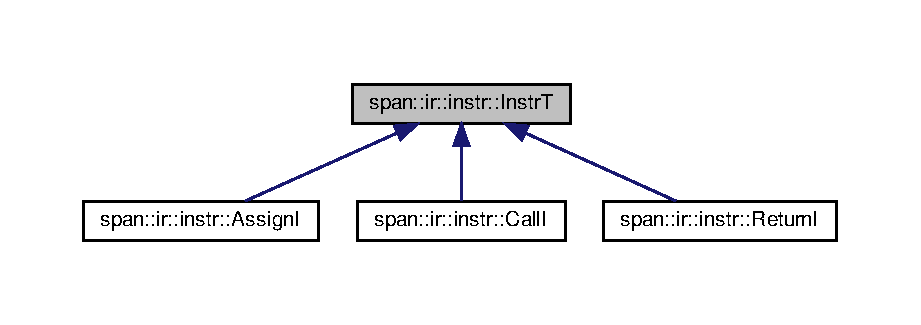
\includegraphics[width=350pt]{classspan_1_1ir_1_1instr_1_1InstrT__inherit__graph}
\end{center}
\end{figure}
\subsection*{Public Member Functions}
\begin{DoxyCompactItemize}
\item 
\mbox{\Hypertarget{classspan_1_1ir_1_1instr_1_1InstrT_ad669661a2dddf4076b70b574340cda89}\label{classspan_1_1ir_1_1instr_1_1InstrT_ad669661a2dddf4076b70b574340cda89}} 
{\bfseries InstrT} (Basic\+Instr\+Kinds Instr\+Code)
\item 
\mbox{\Hypertarget{classspan_1_1ir_1_1instr_1_1InstrT_ad2de1b4476eb459cd511366152ca5a89}\label{classspan_1_1ir_1_1instr_1_1InstrT_ad2de1b4476eb459cd511366152ca5a89}} 
string {\bfseries print} ()
\item 
\mbox{\Hypertarget{classspan_1_1ir_1_1instr_1_1InstrT_afc0c85ffba82d580871e524aa42a951d}\label{classspan_1_1ir_1_1instr_1_1InstrT_afc0c85ffba82d580871e524aa42a951d}} 
{\bfseries InstrT} (Basic\+Instr\+Kinds Instr\+Code)
\end{DoxyCompactItemize}


The documentation for this class was generated from the following files\+:\begin{DoxyCompactItemize}
\item 
Instr (copy).\+h\item 
Instr.\+h\item 
Instr.\+cpp\end{DoxyCompactItemize}

\hypertarget{classspan_1_1ir_1_1types_1_1Record}{}\section{span\+:\+:ir\+:\+:types\+:\+:Record Class Reference}
\label{classspan_1_1ir_1_1types_1_1Record}\index{span\+::ir\+::types\+::\+Record@{span\+::ir\+::types\+::\+Record}}


{\ttfamily \#include $<$types.\+h$>$}



Inheritance diagram for span\+:\+:ir\+:\+:types\+:\+:Record\+:\nopagebreak
\begin{figure}[H]
\begin{center}
\leavevmode
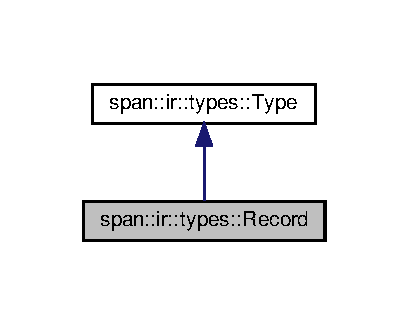
\includegraphics[width=196pt]{classspan_1_1ir_1_1types_1_1Record__inherit__graph}
\end{center}
\end{figure}


Collaboration diagram for span\+:\+:ir\+:\+:types\+:\+:Record\+:\nopagebreak
\begin{figure}[H]
\begin{center}
\leavevmode
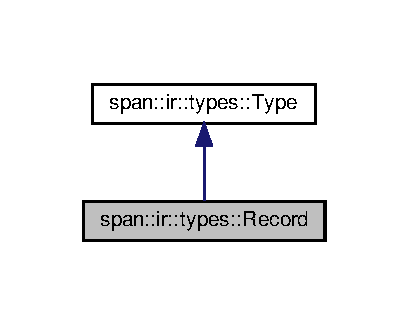
\includegraphics[width=196pt]{classspan_1_1ir_1_1types_1_1Record__coll__graph}
\end{center}
\end{figure}
\subsection*{Private Attributes}
\begin{DoxyCompactItemize}
\item 
bool \hyperlink{classspan_1_1ir_1_1types_1_1Record_a74049e704dca0f9274d322838c284141}{is\+Struct}
\item 
std\+::string \hyperlink{classspan_1_1ir_1_1types_1_1Record_a25b466e4e13c470698683dc9f402bea7}{name}
\item 
std\+::vector$<$ std\+::pair$<$ std\+::string, \hyperlink{classspan_1_1ir_1_1types_1_1Type}{Type} $\ast$ $>$ $>$ \hyperlink{classspan_1_1ir_1_1types_1_1Record_a37a26c710224ad6402ecfb4424369273}{fields}
\end{DoxyCompactItemize}
\subsection*{Additional Inherited Members}


\subsection{Member Data Documentation}
\mbox{\Hypertarget{classspan_1_1ir_1_1types_1_1Record_a37a26c710224ad6402ecfb4424369273}\label{classspan_1_1ir_1_1types_1_1Record_a37a26c710224ad6402ecfb4424369273}} 
\index{span\+::ir\+::types\+::\+Record@{span\+::ir\+::types\+::\+Record}!fields@{fields}}
\index{fields@{fields}!span\+::ir\+::types\+::\+Record@{span\+::ir\+::types\+::\+Record}}
\subsubsection{\texorpdfstring{fields}{fields}}
{\footnotesize\ttfamily std\+::vector$<$std\+::pair$<$std\+::string, \hyperlink{classspan_1_1ir_1_1types_1_1Type}{Type}$\ast$$>$ $>$ span\+::ir\+::types\+::\+Record\+::fields\hspace{0.3cm}{\ttfamily [private]}}

\mbox{\Hypertarget{classspan_1_1ir_1_1types_1_1Record_a74049e704dca0f9274d322838c284141}\label{classspan_1_1ir_1_1types_1_1Record_a74049e704dca0f9274d322838c284141}} 
\index{span\+::ir\+::types\+::\+Record@{span\+::ir\+::types\+::\+Record}!is\+Struct@{is\+Struct}}
\index{is\+Struct@{is\+Struct}!span\+::ir\+::types\+::\+Record@{span\+::ir\+::types\+::\+Record}}
\subsubsection{\texorpdfstring{is\+Struct}{isStruct}}
{\footnotesize\ttfamily bool span\+::ir\+::types\+::\+Record\+::is\+Struct\hspace{0.3cm}{\ttfamily [private]}}

\mbox{\Hypertarget{classspan_1_1ir_1_1types_1_1Record_a25b466e4e13c470698683dc9f402bea7}\label{classspan_1_1ir_1_1types_1_1Record_a25b466e4e13c470698683dc9f402bea7}} 
\index{span\+::ir\+::types\+::\+Record@{span\+::ir\+::types\+::\+Record}!name@{name}}
\index{name@{name}!span\+::ir\+::types\+::\+Record@{span\+::ir\+::types\+::\+Record}}
\subsubsection{\texorpdfstring{name}{name}}
{\footnotesize\ttfamily std\+::string span\+::ir\+::types\+::\+Record\+::name\hspace{0.3cm}{\ttfamily [private]}}



The documentation for this class was generated from the following file\+:\begin{DoxyCompactItemize}
\item 
\hyperlink{types_8h}{types.\+h}\end{DoxyCompactItemize}

\hypertarget{classspan_1_1ir_1_1instr_1_1ReturnI}{}\section{span\+:\+:ir\+:\+:instr\+:\+:ReturnI Class Reference}
\label{classspan_1_1ir_1_1instr_1_1ReturnI}\index{span\+::ir\+::instr\+::\+ReturnI@{span\+::ir\+::instr\+::\+ReturnI}}


Inheritance diagram for span\+:\+:ir\+:\+:instr\+:\+:ReturnI\+:\nopagebreak
\begin{figure}[H]
\begin{center}
\leavevmode
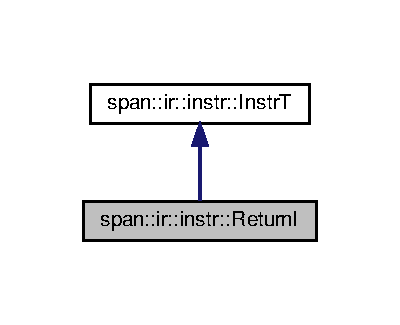
\includegraphics[width=192pt]{classspan_1_1ir_1_1instr_1_1ReturnI__inherit__graph}
\end{center}
\end{figure}


Collaboration diagram for span\+:\+:ir\+:\+:instr\+:\+:ReturnI\+:\nopagebreak
\begin{figure}[H]
\begin{center}
\leavevmode
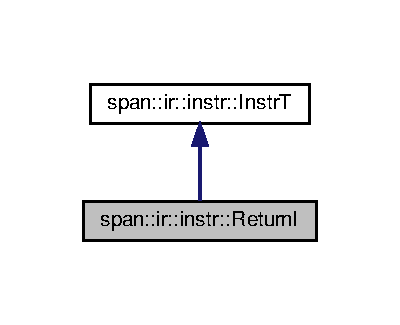
\includegraphics[width=192pt]{classspan_1_1ir_1_1instr_1_1ReturnI__coll__graph}
\end{center}
\end{figure}
\subsection*{Public Member Functions}
\begin{DoxyCompactItemize}
\item 
\mbox{\Hypertarget{classspan_1_1ir_1_1instr_1_1ReturnI_a00200fd821eaaba58d11086181feec45}\label{classspan_1_1ir_1_1instr_1_1ReturnI_a00200fd821eaaba58d11086181feec45}} 
{\bfseries ReturnI} (\hyperlink{classspan_1_1ir_1_1expr_1_1Expr}{expr\+::\+Expr} $\ast$inst)
\item 
\mbox{\Hypertarget{classspan_1_1ir_1_1instr_1_1ReturnI_a14195daefce06ae78a4b7a1ecbacfa37}\label{classspan_1_1ir_1_1instr_1_1ReturnI_a14195daefce06ae78a4b7a1ecbacfa37}} 
string {\bfseries print} ()
\item 
\mbox{\Hypertarget{classspan_1_1ir_1_1instr_1_1ReturnI_a1964d4c5bfcf3ea663309406bc343bcb}\label{classspan_1_1ir_1_1instr_1_1ReturnI_a1964d4c5bfcf3ea663309406bc343bcb}} 
{\bfseries ReturnI} (\hyperlink{classspan_1_1ir_1_1expr_1_1Expr}{expr\+::\+Expr} $\ast$inst)
\end{DoxyCompactItemize}


The documentation for this class was generated from the following files\+:\begin{DoxyCompactItemize}
\item 
Instr (copy).\+h\item 
Instr.\+h\item 
Instr.\+cpp\end{DoxyCompactItemize}

\hypertarget{classspan_1_1ir_1_1tunit_1_1TUnit}{}\section{span\+:\+:ir\+:\+:tunit\+:\+:T\+Unit Class Reference}
\label{classspan_1_1ir_1_1tunit_1_1TUnit}\index{span\+::ir\+::tunit\+::\+T\+Unit@{span\+::ir\+::tunit\+::\+T\+Unit}}


Holds the complete translation unit.  




{\ttfamily \#include $<$T\+Unit (copy).\+h$>$}

\subsection*{Public Member Functions}
\begin{DoxyCompactItemize}
\item 
\mbox{\Hypertarget{classspan_1_1ir_1_1tunit_1_1TUnit_ad6773c50bc2aeaa86815a798ee9ca89d}\label{classspan_1_1ir_1_1tunit_1_1TUnit_ad6773c50bc2aeaa86815a798ee9ca89d}} 
{\bfseries T\+Unit} (std\+::string name, std\+::string description, Var\+Map \&\&var\+Map, Func\+Map func\+Map)
\item 
\mbox{\Hypertarget{classspan_1_1ir_1_1tunit_1_1TUnit_acee42872de33f4c42935d0ee30731234}\label{classspan_1_1ir_1_1tunit_1_1TUnit_acee42872de33f4c42935d0ee30731234}} 
const std\+::string \& \hyperlink{classspan_1_1ir_1_1tunit_1_1TUnit_acee42872de33f4c42935d0ee30731234}{get\+Name} ()
\begin{DoxyCompactList}\small\item\em Get \hyperlink{classspan_1_1ir_1_1tunit_1_1TUnit}{T\+Unit} name, generally the filename. \end{DoxyCompactList}\item 
\mbox{\Hypertarget{classspan_1_1ir_1_1tunit_1_1TUnit_a0376a882680243327f0b3a29a8be58c0}\label{classspan_1_1ir_1_1tunit_1_1TUnit_a0376a882680243327f0b3a29a8be58c0}} 
void \hyperlink{classspan_1_1ir_1_1tunit_1_1TUnit_a0376a882680243327f0b3a29a8be58c0}{set\+Name} (std\+::string name)
\begin{DoxyCompactList}\small\item\em Set \hyperlink{classspan_1_1ir_1_1tunit_1_1TUnit}{T\+Unit} name, generally the filename. \end{DoxyCompactList}\item 
\mbox{\Hypertarget{classspan_1_1ir_1_1tunit_1_1TUnit_ad896bdfde696ce84b09a21eca27ad97d}\label{classspan_1_1ir_1_1tunit_1_1TUnit_ad896bdfde696ce84b09a21eca27ad97d}} 
std\+::string \hyperlink{classspan_1_1ir_1_1tunit_1_1TUnit_ad896bdfde696ce84b09a21eca27ad97d}{get\+Description} ()
\begin{DoxyCompactList}\small\item\em Get \hyperlink{classspan_1_1ir_1_1tunit_1_1TUnit}{T\+Unit} (optional) description. \end{DoxyCompactList}\item 
void \hyperlink{classspan_1_1ir_1_1tunit_1_1TUnit_a7282396b2197abecf4be7b83232de887}{set\+Description} (std\+::string description)
\item 
\mbox{\Hypertarget{classspan_1_1ir_1_1tunit_1_1TUnit_a8a459d7ce6e0bea270c6a5b85dd760d3}\label{classspan_1_1ir_1_1tunit_1_1TUnit_a8a459d7ce6e0bea270c6a5b85dd760d3}} 
std\+::vector$<$ string $>$ {\bfseries Ret\+\_\+\+String} ()
\item 
\mbox{\Hypertarget{classspan_1_1ir_1_1tunit_1_1TUnit_a38b571a7c30b503bc67a2c64f0f9f8b8}\label{classspan_1_1ir_1_1tunit_1_1TUnit_a38b571a7c30b503bc67a2c64f0f9f8b8}} 
{\bfseries T\+Unit} (std\+::string name, std\+::string description, Var\+Map \&\&var\+Map, Func\+Map func\+Map)
\item 
\mbox{\Hypertarget{classspan_1_1ir_1_1tunit_1_1TUnit_a2a224cfa26d81e169f2b3b36e3176562}\label{classspan_1_1ir_1_1tunit_1_1TUnit_a2a224cfa26d81e169f2b3b36e3176562}} 
const std\+::string \& \hyperlink{classspan_1_1ir_1_1tunit_1_1TUnit_a2a224cfa26d81e169f2b3b36e3176562}{get\+Name} ()
\begin{DoxyCompactList}\small\item\em Get \hyperlink{classspan_1_1ir_1_1tunit_1_1TUnit}{T\+Unit} name, generally the filename. \end{DoxyCompactList}\item 
\mbox{\Hypertarget{classspan_1_1ir_1_1tunit_1_1TUnit_aafb230fac04e8d88606257223a21d198}\label{classspan_1_1ir_1_1tunit_1_1TUnit_aafb230fac04e8d88606257223a21d198}} 
void \hyperlink{classspan_1_1ir_1_1tunit_1_1TUnit_aafb230fac04e8d88606257223a21d198}{set\+Name} (std\+::string name)
\begin{DoxyCompactList}\small\item\em Set \hyperlink{classspan_1_1ir_1_1tunit_1_1TUnit}{T\+Unit} name, generally the filename. \end{DoxyCompactList}\item 
\mbox{\Hypertarget{classspan_1_1ir_1_1tunit_1_1TUnit_ae80082eafb1c5ab45732473730d681a8}\label{classspan_1_1ir_1_1tunit_1_1TUnit_ae80082eafb1c5ab45732473730d681a8}} 
std\+::string \hyperlink{classspan_1_1ir_1_1tunit_1_1TUnit_ae80082eafb1c5ab45732473730d681a8}{get\+Description} ()
\begin{DoxyCompactList}\small\item\em Get \hyperlink{classspan_1_1ir_1_1tunit_1_1TUnit}{T\+Unit} (optional) description. \end{DoxyCompactList}\item 
void \hyperlink{classspan_1_1ir_1_1tunit_1_1TUnit_a74ebf1c50b498f8117a9fd9257ad501d}{set\+Description} (std\+::string description)
\item 
\mbox{\Hypertarget{classspan_1_1ir_1_1tunit_1_1TUnit_aadc76e7e08bf3b9a0f8be5a7ef339783}\label{classspan_1_1ir_1_1tunit_1_1TUnit_aadc76e7e08bf3b9a0f8be5a7ef339783}} 
void {\bfseries show} ()
\end{DoxyCompactItemize}


\subsection{Detailed Description}
Holds the complete translation unit. 

\subsection{Member Function Documentation}
\mbox{\Hypertarget{classspan_1_1ir_1_1tunit_1_1TUnit_a7282396b2197abecf4be7b83232de887}\label{classspan_1_1ir_1_1tunit_1_1TUnit_a7282396b2197abecf4be7b83232de887}} 
\index{span\+::ir\+::tunit\+::\+T\+Unit@{span\+::ir\+::tunit\+::\+T\+Unit}!set\+Description@{set\+Description}}
\index{set\+Description@{set\+Description}!span\+::ir\+::tunit\+::\+T\+Unit@{span\+::ir\+::tunit\+::\+T\+Unit}}
\subsubsection{\texorpdfstring{set\+Description()}{setDescription()}\hspace{0.1cm}{\footnotesize\ttfamily [1/2]}}
{\footnotesize\ttfamily void T\+Unit\+::set\+Description (\begin{DoxyParamCaption}\item[{std\+::string}]{description }\end{DoxyParamCaption})}

Set \hyperlink{classspan_1_1ir_1_1tunit_1_1TUnit}{T\+Unit} (optional) description 
\begin{DoxyParams}{Parameters}
{\em description} & an optional description of the translation unit \\
\hline
\end{DoxyParams}
\mbox{\Hypertarget{classspan_1_1ir_1_1tunit_1_1TUnit_a74ebf1c50b498f8117a9fd9257ad501d}\label{classspan_1_1ir_1_1tunit_1_1TUnit_a74ebf1c50b498f8117a9fd9257ad501d}} 
\index{span\+::ir\+::tunit\+::\+T\+Unit@{span\+::ir\+::tunit\+::\+T\+Unit}!set\+Description@{set\+Description}}
\index{set\+Description@{set\+Description}!span\+::ir\+::tunit\+::\+T\+Unit@{span\+::ir\+::tunit\+::\+T\+Unit}}
\subsubsection{\texorpdfstring{set\+Description()}{setDescription()}\hspace{0.1cm}{\footnotesize\ttfamily [2/2]}}
{\footnotesize\ttfamily void span\+::ir\+::tunit\+::\+T\+Unit\+::set\+Description (\begin{DoxyParamCaption}\item[{std\+::string}]{description }\end{DoxyParamCaption})}

Set \hyperlink{classspan_1_1ir_1_1tunit_1_1TUnit}{T\+Unit} (optional) description 
\begin{DoxyParams}{Parameters}
{\em description} & an optional description of the translation unit \\
\hline
\end{DoxyParams}


The documentation for this class was generated from the following files\+:\begin{DoxyCompactItemize}
\item 
T\+Unit (copy).\+h\item 
T\+Unit.\+h\item 
T\+Unit.\+cpp\end{DoxyCompactItemize}

\hypertarget{classspan_1_1ir_1_1types_1_1Type}{}\section{span\+:\+:ir\+:\+:types\+:\+:Type Class Reference}
\label{classspan_1_1ir_1_1types_1_1Type}\index{span\+::ir\+::types\+::\+Type@{span\+::ir\+::types\+::\+Type}}


Inheritance diagram for span\+:\+:ir\+:\+:types\+:\+:Type\+:\nopagebreak
\begin{figure}[H]
\begin{center}
\leavevmode
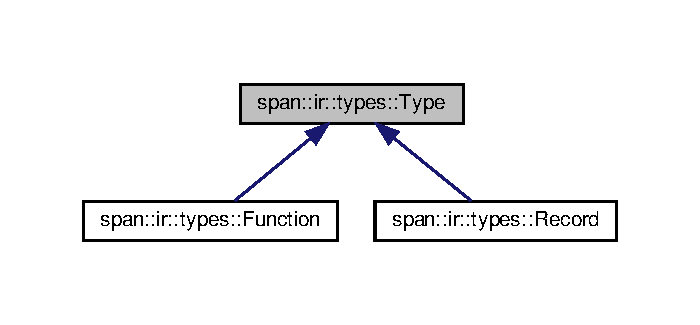
\includegraphics[width=350pt]{classspan_1_1ir_1_1types_1_1Type__inherit__graph}
\end{center}
\end{figure}
\subsection*{Public Member Functions}
\begin{DoxyCompactItemize}
\item 
\mbox{\Hypertarget{classspan_1_1ir_1_1types_1_1Type_ab951af2db49103cbccf8374a26ee5fcb}\label{classspan_1_1ir_1_1types_1_1Type_ab951af2db49103cbccf8374a26ee5fcb}} 
{\bfseries Type} (Basic\+Type\+Kinds type\+Code)
\item 
\mbox{\Hypertarget{classspan_1_1ir_1_1types_1_1Type_afbf3f9699ba99a890d71f3d32e34e682}\label{classspan_1_1ir_1_1types_1_1Type_afbf3f9699ba99a890d71f3d32e34e682}} 
Basic\+Type\+Kinds {\bfseries get\+Type\+Code} ()
\item 
\mbox{\Hypertarget{classspan_1_1ir_1_1types_1_1Type_a891e98af6fbffc2ff6e278f123e6ff48}\label{classspan_1_1ir_1_1types_1_1Type_a891e98af6fbffc2ff6e278f123e6ff48}} 
virtual string {\bfseries print} ()
\item 
\mbox{\Hypertarget{classspan_1_1ir_1_1types_1_1Type_a3170f3a05d7580ad72410ff3a6a8bfd7}\label{classspan_1_1ir_1_1types_1_1Type_a3170f3a05d7580ad72410ff3a6a8bfd7}} 
bool {\bfseries is\+Integer} ()
\item 
\mbox{\Hypertarget{classspan_1_1ir_1_1types_1_1Type_a3ba754a44b1fe841cca197a7ec3bf325}\label{classspan_1_1ir_1_1types_1_1Type_a3ba754a44b1fe841cca197a7ec3bf325}} 
bool {\bfseries is\+Unsigned} ()
\item 
\mbox{\Hypertarget{classspan_1_1ir_1_1types_1_1Type_af00ec0e491278804eaf6a54f972200cf}\label{classspan_1_1ir_1_1types_1_1Type_af00ec0e491278804eaf6a54f972200cf}} 
bool {\bfseries is\+Float} ()
\item 
\mbox{\Hypertarget{classspan_1_1ir_1_1types_1_1Type_ac833373012206ec5add217b6be11a8a3}\label{classspan_1_1ir_1_1types_1_1Type_ac833373012206ec5add217b6be11a8a3}} 
bool {\bfseries is\+Numeric} ()
\item 
\mbox{\Hypertarget{classspan_1_1ir_1_1types_1_1Type_a3aa56f9fce97ff1762575d5ca8b9759d}\label{classspan_1_1ir_1_1types_1_1Type_a3aa56f9fce97ff1762575d5ca8b9759d}} 
bool {\bfseries is\+Pointer} ()
\item 
\mbox{\Hypertarget{classspan_1_1ir_1_1types_1_1Type_ab7ade487742cde86e00e3d8235484656}\label{classspan_1_1ir_1_1types_1_1Type_ab7ade487742cde86e00e3d8235484656}} 
bool {\bfseries is\+Func} ()
\item 
\mbox{\Hypertarget{classspan_1_1ir_1_1types_1_1Type_aa53eda1db929768a1fea0f696ba2ba10}\label{classspan_1_1ir_1_1types_1_1Type_aa53eda1db929768a1fea0f696ba2ba10}} 
bool {\bfseries is\+Struct} ()
\item 
\mbox{\Hypertarget{classspan_1_1ir_1_1types_1_1Type_a949e9e027abf854bf1714ae02a078a5e}\label{classspan_1_1ir_1_1types_1_1Type_a949e9e027abf854bf1714ae02a078a5e}} 
bool {\bfseries is\+Void} ()
\item 
\mbox{\Hypertarget{classspan_1_1ir_1_1types_1_1Type_a3f6163fcc2aa87bb104ed94d0f3212b9}\label{classspan_1_1ir_1_1types_1_1Type_a3f6163fcc2aa87bb104ed94d0f3212b9}} 
{\bfseries Type} (Basic\+Type\+Kinds type\+Code)
\item 
\mbox{\Hypertarget{classspan_1_1ir_1_1types_1_1Type_a9e13548ef5aa1f44aeb65b6e5cac6893}\label{classspan_1_1ir_1_1types_1_1Type_a9e13548ef5aa1f44aeb65b6e5cac6893}} 
Basic\+Type\+Kinds {\bfseries get\+Type\+Code} ()
\item 
\mbox{\Hypertarget{classspan_1_1ir_1_1types_1_1Type_a60731408750a7f723c7fe23ac13a9260}\label{classspan_1_1ir_1_1types_1_1Type_a60731408750a7f723c7fe23ac13a9260}} 
virtual void {\bfseries print} ()
\item 
\mbox{\Hypertarget{classspan_1_1ir_1_1types_1_1Type_a70459a5409a57db4850aa0e2715afcbb}\label{classspan_1_1ir_1_1types_1_1Type_a70459a5409a57db4850aa0e2715afcbb}} 
bool {\bfseries is\+Integer} ()
\item 
\mbox{\Hypertarget{classspan_1_1ir_1_1types_1_1Type_a61193131f53ef462f0d2597c3a3aa672}\label{classspan_1_1ir_1_1types_1_1Type_a61193131f53ef462f0d2597c3a3aa672}} 
bool {\bfseries is\+Unsigned} ()
\item 
\mbox{\Hypertarget{classspan_1_1ir_1_1types_1_1Type_a54000c25eb3f6846047f0b3e721b7b1e}\label{classspan_1_1ir_1_1types_1_1Type_a54000c25eb3f6846047f0b3e721b7b1e}} 
bool {\bfseries is\+Float} ()
\item 
\mbox{\Hypertarget{classspan_1_1ir_1_1types_1_1Type_aefda2054996b62f24684ba759319c30d}\label{classspan_1_1ir_1_1types_1_1Type_aefda2054996b62f24684ba759319c30d}} 
bool {\bfseries is\+Numeric} ()
\item 
\mbox{\Hypertarget{classspan_1_1ir_1_1types_1_1Type_a80171ad0549f9175f9f4e2ebd6680b63}\label{classspan_1_1ir_1_1types_1_1Type_a80171ad0549f9175f9f4e2ebd6680b63}} 
bool {\bfseries is\+Pointer} ()
\item 
\mbox{\Hypertarget{classspan_1_1ir_1_1types_1_1Type_aa42ffaf20d7608233d71b92d269775ea}\label{classspan_1_1ir_1_1types_1_1Type_aa42ffaf20d7608233d71b92d269775ea}} 
bool {\bfseries is\+Func} ()
\item 
\mbox{\Hypertarget{classspan_1_1ir_1_1types_1_1Type_a4c26d42aa7df67c2bdd6ba1069a84650}\label{classspan_1_1ir_1_1types_1_1Type_a4c26d42aa7df67c2bdd6ba1069a84650}} 
bool {\bfseries is\+Struct} ()
\item 
\mbox{\Hypertarget{classspan_1_1ir_1_1types_1_1Type_a0271017ec818928be7103216039bc2b5}\label{classspan_1_1ir_1_1types_1_1Type_a0271017ec818928be7103216039bc2b5}} 
bool {\bfseries is\+Void} ()
\end{DoxyCompactItemize}


The documentation for this class was generated from the following files\+:\begin{DoxyCompactItemize}
\item 
Types (copy).\+h\item 
Types.\+h\item 
Types.\+cpp\end{DoxyCompactItemize}

\hypertarget{classspan_1_1ir_1_1expr_1_1UnaryExpr}{}\section{span\+:\+:ir\+:\+:expr\+:\+:Unary\+Expr Class Reference}
\label{classspan_1_1ir_1_1expr_1_1UnaryExpr}\index{span\+::ir\+::expr\+::\+Unary\+Expr@{span\+::ir\+::expr\+::\+Unary\+Expr}}


Inheritance diagram for span\+:\+:ir\+:\+:expr\+:\+:Unary\+Expr\+:\nopagebreak
\begin{figure}[H]
\begin{center}
\leavevmode
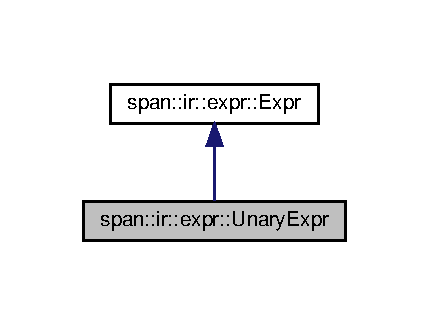
\includegraphics[width=206pt]{classspan_1_1ir_1_1expr_1_1UnaryExpr__inherit__graph}
\end{center}
\end{figure}


Collaboration diagram for span\+:\+:ir\+:\+:expr\+:\+:Unary\+Expr\+:\nopagebreak
\begin{figure}[H]
\begin{center}
\leavevmode
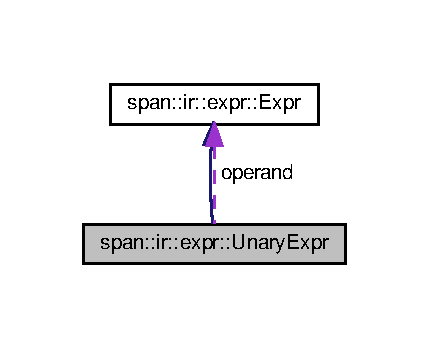
\includegraphics[width=298pt]{classspan_1_1ir_1_1expr_1_1UnaryExpr__coll__graph}
\end{center}
\end{figure}
\subsection*{Public Member Functions}
\begin{DoxyCompactItemize}
\item 
\mbox{\Hypertarget{classspan_1_1ir_1_1expr_1_1UnaryExpr_aef18ea3acac2a31dd3ce664eb42deadd}\label{classspan_1_1ir_1_1expr_1_1UnaryExpr_aef18ea3acac2a31dd3ce664eb42deadd}} 
{\bfseries Unary\+Expr} (\hyperlink{namespacespan_1_1ir_1_1op_ab88ceb1213c3473d4f5fc848509dd181}{op\+::\+Unary\+Operator\+Kind} op\+Code, \hyperlink{classspan_1_1ir_1_1expr_1_1UnitExpr}{Unit\+Expr} $\ast$operand)
\item 
\mbox{\Hypertarget{classspan_1_1ir_1_1expr_1_1UnaryExpr_a6b8567c35a7b96f909bff41e13d601bf}\label{classspan_1_1ir_1_1expr_1_1UnaryExpr_a6b8567c35a7b96f909bff41e13d601bf}} 
{\bfseries Unary\+Expr} (\hyperlink{namespacespan_1_1ir_1_1op_ab88ceb1213c3473d4f5fc848509dd181}{op\+::\+Unary\+Operator\+Kind} op\+Code, \hyperlink{classspan_1_1ir_1_1expr_1_1UnitExpr}{Unit\+Expr} $\ast$operand)
\end{DoxyCompactItemize}
\subsection*{Public Attributes}
\begin{DoxyCompactItemize}
\item 
\mbox{\Hypertarget{classspan_1_1ir_1_1expr_1_1UnaryExpr_a7074043b3e6e97557ef1df01e93a26e6}\label{classspan_1_1ir_1_1expr_1_1UnaryExpr_a7074043b3e6e97557ef1df01e93a26e6}} 
\hyperlink{namespacespan_1_1ir_1_1op_ab88ceb1213c3473d4f5fc848509dd181}{op\+::\+Unary\+Operator\+Kind} {\bfseries op\+Code}
\item 
\mbox{\Hypertarget{classspan_1_1ir_1_1expr_1_1UnaryExpr_ac05be81012d5faff7afe5a626c3eec8f}\label{classspan_1_1ir_1_1expr_1_1UnaryExpr_ac05be81012d5faff7afe5a626c3eec8f}} 
\hyperlink{classspan_1_1ir_1_1expr_1_1UnitExpr}{Unit\+Expr} $\ast$ {\bfseries operand}
\end{DoxyCompactItemize}


The documentation for this class was generated from the following files\+:\begin{DoxyCompactItemize}
\item 
Expr (copy).\+h\item 
Expr.\+h\item 
Expr.\+cpp\end{DoxyCompactItemize}

\hypertarget{classspan_1_1ir_1_1expr_1_1UnitExpr}{}\section{span\+:\+:ir\+:\+:expr\+:\+:Unit\+Expr Class Reference}
\label{classspan_1_1ir_1_1expr_1_1UnitExpr}\index{span\+::ir\+::expr\+::\+Unit\+Expr@{span\+::ir\+::expr\+::\+Unit\+Expr}}


{\ttfamily \#include $<$expr.\+h$>$}



Inheritance diagram for span\+:\+:ir\+:\+:expr\+:\+:Unit\+Expr\+:\nopagebreak
\begin{figure}[H]
\begin{center}
\leavevmode
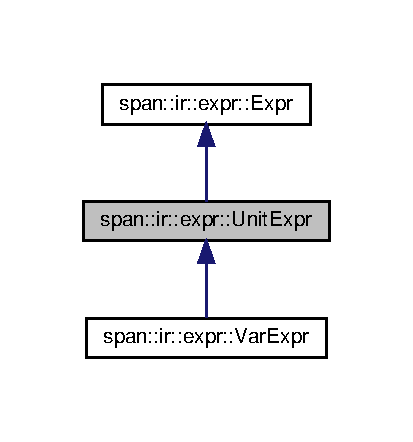
\includegraphics[width=198pt]{classspan_1_1ir_1_1expr_1_1UnitExpr__inherit__graph}
\end{center}
\end{figure}


Collaboration diagram for span\+:\+:ir\+:\+:expr\+:\+:Unit\+Expr\+:\nopagebreak
\begin{figure}[H]
\begin{center}
\leavevmode
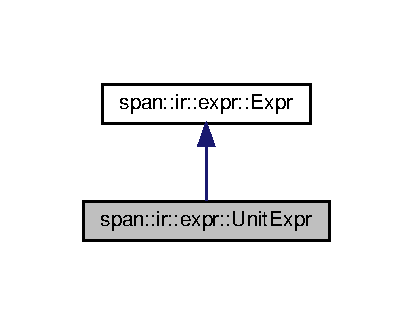
\includegraphics[width=198pt]{classspan_1_1ir_1_1expr_1_1UnitExpr__coll__graph}
\end{center}
\end{figure}


The documentation for this class was generated from the following file\+:\begin{DoxyCompactItemize}
\item 
\hyperlink{expr_8h}{expr.\+h}\end{DoxyCompactItemize}

\hypertarget{classspan_1_1ir_1_1expr_1_1VarExpr}{}\section{span\+:\+:ir\+:\+:expr\+:\+:Var\+Expr Class Reference}
\label{classspan_1_1ir_1_1expr_1_1VarExpr}\index{span\+::ir\+::expr\+::\+Var\+Expr@{span\+::ir\+::expr\+::\+Var\+Expr}}


{\ttfamily \#include $<$expr.\+h$>$}



Inheritance diagram for span\+:\+:ir\+:\+:expr\+:\+:Var\+Expr\+:\nopagebreak
\begin{figure}[H]
\begin{center}
\leavevmode
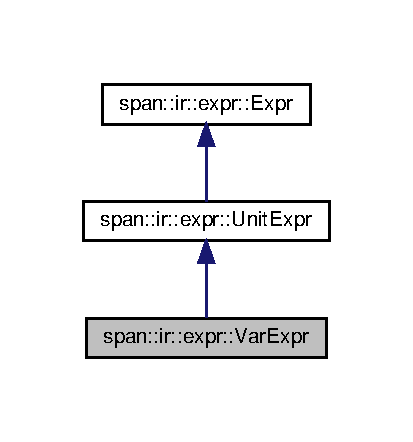
\includegraphics[width=198pt]{classspan_1_1ir_1_1expr_1_1VarExpr__inherit__graph}
\end{center}
\end{figure}


Collaboration diagram for span\+:\+:ir\+:\+:expr\+:\+:Var\+Expr\+:\nopagebreak
\begin{figure}[H]
\begin{center}
\leavevmode
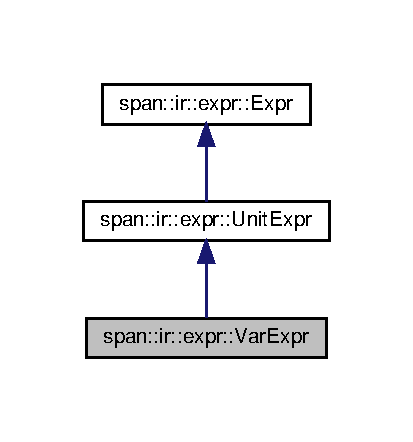
\includegraphics[width=198pt]{classspan_1_1ir_1_1expr_1_1VarExpr__coll__graph}
\end{center}
\end{figure}
\subsection*{Private Attributes}
\begin{DoxyCompactItemize}
\item 
std\+::string \hyperlink{classspan_1_1ir_1_1expr_1_1VarExpr_a03e1f8d576b09c4745e093bf464d0347}{name}
\end{DoxyCompactItemize}


\subsection{Member Data Documentation}
\mbox{\Hypertarget{classspan_1_1ir_1_1expr_1_1VarExpr_a03e1f8d576b09c4745e093bf464d0347}\label{classspan_1_1ir_1_1expr_1_1VarExpr_a03e1f8d576b09c4745e093bf464d0347}} 
\index{span\+::ir\+::expr\+::\+Var\+Expr@{span\+::ir\+::expr\+::\+Var\+Expr}!name@{name}}
\index{name@{name}!span\+::ir\+::expr\+::\+Var\+Expr@{span\+::ir\+::expr\+::\+Var\+Expr}}
\subsubsection{\texorpdfstring{name}{name}}
{\footnotesize\ttfamily std\+::string span\+::ir\+::expr\+::\+Var\+Expr\+::name\hspace{0.3cm}{\ttfamily [private]}}



The documentation for this class was generated from the following file\+:\begin{DoxyCompactItemize}
\item 
\hyperlink{expr_8h}{expr.\+h}\end{DoxyCompactItemize}

\chapter{File Documentation}
\hypertarget{docs_8h}{}\section{docs.\+h File Reference}
\label{docs_8h}\index{docs.\+h@{docs.\+h}}

\hypertarget{expr_8h}{}\section{expr.\+h File Reference}
\label{expr_8h}\index{expr.\+h@{expr.\+h}}
{\ttfamily \#include \char`\"{}op\+Kinds.\+h\char`\"{}}\newline
Include dependency graph for expr.\+h\+:\nopagebreak
\begin{figure}[H]
\begin{center}
\leavevmode
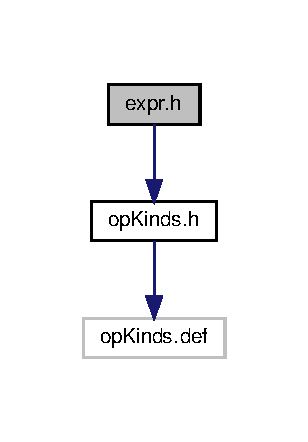
\includegraphics[width=148pt]{expr_8h__incl}
\end{center}
\end{figure}
This graph shows which files directly or indirectly include this file\+:\nopagebreak
\begin{figure}[H]
\begin{center}
\leavevmode
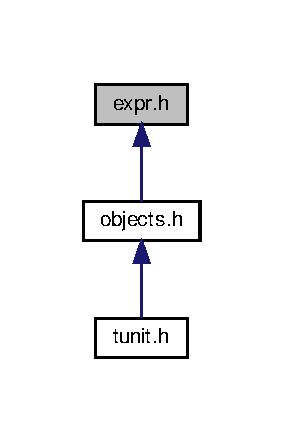
\includegraphics[width=136pt]{expr_8h__dep__incl}
\end{center}
\end{figure}
\subsection*{Classes}
\begin{DoxyCompactItemize}
\item 
class \hyperlink{classspan_1_1ir_1_1expr_1_1Expr}{span\+::ir\+::expr\+::\+Expr}
\item 
class \hyperlink{classspan_1_1ir_1_1expr_1_1UnitExpr}{span\+::ir\+::expr\+::\+Unit\+Expr}
\item 
class \hyperlink{classspan_1_1ir_1_1expr_1_1VarExpr}{span\+::ir\+::expr\+::\+Var\+Expr}
\item 
class \hyperlink{classspan_1_1ir_1_1expr_1_1BinaryExpr}{span\+::ir\+::expr\+::\+Binary\+Expr}
\item 
class \hyperlink{classspan_1_1ir_1_1expr_1_1UnaryExpr}{span\+::ir\+::expr\+::\+Unary\+Expr}
\end{DoxyCompactItemize}
\subsection*{Namespaces}
\begin{DoxyCompactItemize}
\item 
 \hyperlink{namespacespan}{span}
\begin{DoxyCompactList}\small\item\em Encapsulates all of S\+P\+AN. \end{DoxyCompactList}\item 
 \hyperlink{namespacespan_1_1ir}{span\+::ir}
\begin{DoxyCompactList}\small\item\em Contains all of S\+P\+AN IR. \end{DoxyCompactList}\item 
 \hyperlink{namespacespan_1_1ir_1_1expr}{span\+::ir\+::expr}
\begin{DoxyCompactList}\small\item\em The expressions used in instructions. \end{DoxyCompactList}\end{DoxyCompactItemize}

\hypertarget{instr_8h}{}\section{instr.\+h File Reference}
\label{instr_8h}\index{instr.\+h@{instr.\+h}}
This graph shows which files directly or indirectly include this file\+:\nopagebreak
\begin{figure}[H]
\begin{center}
\leavevmode
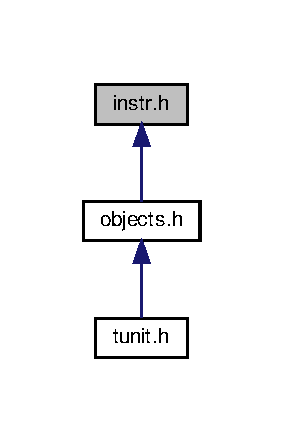
\includegraphics[width=136pt]{instr_8h__dep__incl}
\end{center}
\end{figure}
\subsection*{Classes}
\begin{DoxyCompactItemize}
\item 
class \hyperlink{classspan_1_1ir_1_1instr_1_1InstrT}{span\+::ir\+::instr\+::\+InstrT}
\item 
class \hyperlink{classspan_1_1ir_1_1instr_1_1AssignI}{span\+::ir\+::instr\+::\+AssignI}
\item 
class \hyperlink{classspan_1_1ir_1_1instr_1_1CallI}{span\+::ir\+::instr\+::\+CallI}
\item 
class \hyperlink{classspan_1_1ir_1_1instr_1_1ReturnI}{span\+::ir\+::instr\+::\+ReturnI}
\end{DoxyCompactItemize}
\subsection*{Namespaces}
\begin{DoxyCompactItemize}
\item 
 \hyperlink{namespacespan}{span}
\begin{DoxyCompactList}\small\item\em Encapsulates all of S\+P\+AN. \end{DoxyCompactList}\item 
 \hyperlink{namespacespan_1_1ir}{span\+::ir}
\begin{DoxyCompactList}\small\item\em Contains all of S\+P\+AN IR. \end{DoxyCompactList}\item 
 \hyperlink{namespacespan_1_1ir_1_1instr}{span\+::ir\+::instr}
\begin{DoxyCompactList}\small\item\em The instructions (three-\/address). \end{DoxyCompactList}\end{DoxyCompactItemize}

\hypertarget{library_8cpp}{}\section{library.\+cpp File Reference}
\label{library_8cpp}\index{library.\+cpp@{library.\+cpp}}
{\ttfamily \#include \char`\"{}library.\+h\char`\"{}}\newline
{\ttfamily \#include $<$iostream$>$}\newline
Include dependency graph for library.\+cpp\+:\nopagebreak
\begin{figure}[H]
\begin{center}
\leavevmode
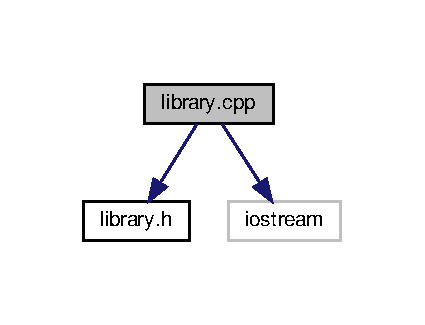
\includegraphics[width=204pt]{library_8cpp__incl}
\end{center}
\end{figure}
\subsection*{Functions}
\begin{DoxyCompactItemize}
\item 
void \hyperlink{library_8cpp_a27a1864e1f4693766ae2596e6e205731}{hello} ()
\end{DoxyCompactItemize}


\subsection{Function Documentation}
\mbox{\Hypertarget{library_8cpp_a27a1864e1f4693766ae2596e6e205731}\label{library_8cpp_a27a1864e1f4693766ae2596e6e205731}} 
\index{library.\+cpp@{library.\+cpp}!hello@{hello}}
\index{hello@{hello}!library.\+cpp@{library.\+cpp}}
\subsubsection{\texorpdfstring{hello()}{hello()}}
{\footnotesize\ttfamily void hello (\begin{DoxyParamCaption}{ }\end{DoxyParamCaption})}


\hypertarget{library_8h}{}\section{library.\+h File Reference}
\label{library_8h}\index{library.\+h@{library.\+h}}
This graph shows which files directly or indirectly include this file\+:\nopagebreak
\begin{figure}[H]
\begin{center}
\leavevmode
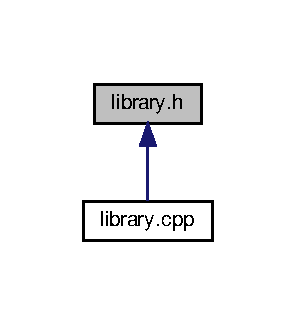
\includegraphics[width=142pt]{library_8h__dep__incl}
\end{center}
\end{figure}
\subsection*{Functions}
\begin{DoxyCompactItemize}
\item 
void \hyperlink{library_8h_a27a1864e1f4693766ae2596e6e205731}{hello} ()
\end{DoxyCompactItemize}


\subsection{Function Documentation}
\mbox{\Hypertarget{library_8h_a27a1864e1f4693766ae2596e6e205731}\label{library_8h_a27a1864e1f4693766ae2596e6e205731}} 
\index{library.\+h@{library.\+h}!hello@{hello}}
\index{hello@{hello}!library.\+h@{library.\+h}}
\subsubsection{\texorpdfstring{hello()}{hello()}}
{\footnotesize\ttfamily void hello (\begin{DoxyParamCaption}{ }\end{DoxyParamCaption})}


\hypertarget{objects_8h}{}\section{objects.\+h File Reference}
\label{objects_8h}\index{objects.\+h@{objects.\+h}}
{\ttfamily \#include $<$unordered\+\_\+map$>$}\newline
{\ttfamily \#include $<$vector$>$}\newline
{\ttfamily \#include \char`\"{}types.\+h\char`\"{}}\newline
{\ttfamily \#include \char`\"{}op\+Kinds.\+h\char`\"{}}\newline
{\ttfamily \#include \char`\"{}instr.\+h\char`\"{}}\newline
{\ttfamily \#include \char`\"{}expr.\+h\char`\"{}}\newline
Include dependency graph for objects.\+h\+:\nopagebreak
\begin{figure}[H]
\begin{center}
\leavevmode
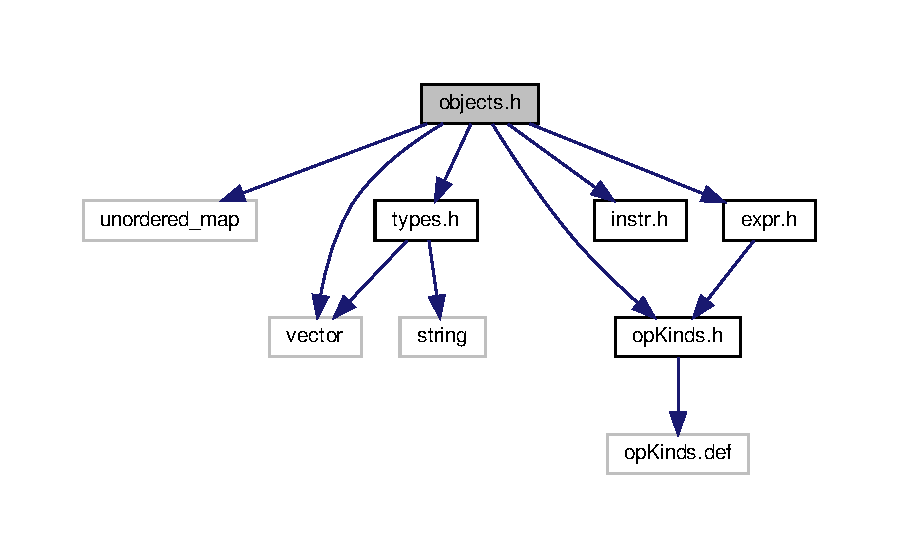
\includegraphics[width=350pt]{objects_8h__incl}
\end{center}
\end{figure}
This graph shows which files directly or indirectly include this file\+:\nopagebreak
\begin{figure}[H]
\begin{center}
\leavevmode
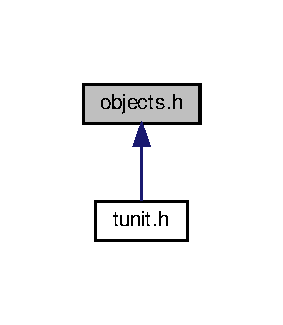
\includegraphics[width=136pt]{objects_8h__dep__incl}
\end{center}
\end{figure}
\subsection*{Classes}
\begin{DoxyCompactItemize}
\item 
class \hyperlink{classspan_1_1ir_1_1obj_1_1BB}{span\+::ir\+::obj\+::\+BB}
\begin{DoxyCompactList}\small\item\em A basic block containing a sequence of instructions. \end{DoxyCompactList}\item 
class \hyperlink{classspan_1_1ir_1_1obj_1_1BBEdge}{span\+::ir\+::obj\+::\+B\+B\+Edge}
\begin{DoxyCompactList}\small\item\em A labeled edge connecting basic blocks. \end{DoxyCompactList}\item 
class \hyperlink{classspan_1_1ir_1_1obj_1_1CFGNode}{span\+::ir\+::obj\+::\+C\+F\+G\+Node}
\begin{DoxyCompactList}\small\item\em A \hyperlink{classspan_1_1ir_1_1obj_1_1CFG}{C\+FG} Node. \end{DoxyCompactList}\item 
class \hyperlink{classspan_1_1ir_1_1obj_1_1CFGNodeEdge}{span\+::ir\+::obj\+::\+C\+F\+G\+Node\+Edge}
\begin{DoxyCompactList}\small\item\em A labeled edge connecting \hyperlink{classspan_1_1ir_1_1obj_1_1CFG}{C\+FG} Nodes. \end{DoxyCompactList}\item 
class \hyperlink{classspan_1_1ir_1_1obj_1_1CFG}{span\+::ir\+::obj\+::\+C\+FG}
\begin{DoxyCompactList}\small\item\em Control Flow Graph. \end{DoxyCompactList}\item 
class \hyperlink{classspan_1_1ir_1_1obj_1_1Function}{span\+::ir\+::obj\+::\+Function}
\begin{DoxyCompactList}\small\item\em A function declaration/definition. \end{DoxyCompactList}\end{DoxyCompactItemize}
\subsection*{Namespaces}
\begin{DoxyCompactItemize}
\item 
 \hyperlink{namespacespan}{span}
\begin{DoxyCompactList}\small\item\em Encapsulates all of S\+P\+AN. \end{DoxyCompactList}\item 
 \hyperlink{namespacespan_1_1ir}{span\+::ir}
\begin{DoxyCompactList}\small\item\em Contains all of S\+P\+AN IR. \end{DoxyCompactList}\item 
 \hyperlink{namespacespan_1_1ir_1_1obj}{span\+::ir\+::obj}
\begin{DoxyCompactList}\small\item\em Objects in a translation unit. \end{DoxyCompactList}\end{DoxyCompactItemize}
\subsection*{Typedefs}
\begin{DoxyCompactItemize}
\item 
typedef std\+::pair$<$ Basic\+Block\+Id, std\+::pair$<$ Basic\+Block\+Id, Edge\+Kind $>$ $>$ \hyperlink{namespacespan_1_1ir_1_1obj_a67ae67fe77ea84d3152bc68919e50c7f}{span\+::ir\+::obj\+::\+B\+B\+Id\+Edge}
\begin{DoxyCompactList}\small\item\em Edge from bb id to bb id (useful for serialization/deserialization) \end{DoxyCompactList}\item 
typedef std\+::pair$<$ C\+F\+G\+Node\+Id, std\+::pair$<$ C\+F\+G\+Node\+Id, Edge\+Kind $>$ $>$ \hyperlink{namespacespan_1_1ir_1_1obj_a8896662ab566cd79d401c0753d3c4120}{span\+::ir\+::obj\+::\+C\+F\+G\+Node\+Id\+Edge}
\begin{DoxyCompactList}\small\item\em Edge from \hyperlink{classspan_1_1ir_1_1obj_1_1CFGNode}{C\+F\+G\+Node} id to \hyperlink{classspan_1_1ir_1_1obj_1_1CFGNode}{C\+F\+G\+Node} id (useful for serialization/deserialization) \end{DoxyCompactList}\end{DoxyCompactItemize}
\subsection*{Enumerations}
\begin{DoxyCompactItemize}
\item 
enum \hyperlink{namespacespan_1_1ir_1_1obj_a3687553dc31f18fb1bd62e0798a3f7f0}{span\+::ir\+::obj\+::\+Edge\+Kind} \{ \hyperlink{namespacespan_1_1ir_1_1obj_a3687553dc31f18fb1bd62e0798a3f7f0a1f5ee4019ffe09583948f65d14d7afce}{span\+::ir\+::obj\+::\+F\+A\+L\+S\+E\+\_\+\+E\+D\+GE}, 
\hyperlink{namespacespan_1_1ir_1_1obj_a3687553dc31f18fb1bd62e0798a3f7f0a233ed7b2a720909aa5557ba66d0fb25c}{span\+::ir\+::obj\+::\+T\+R\+U\+E\+\_\+\+E\+D\+GE}, 
\hyperlink{namespacespan_1_1ir_1_1obj_a3687553dc31f18fb1bd62e0798a3f7f0adc309b8217eea09bb5438dba823068c6}{span\+::ir\+::obj\+::\+U\+N\+C\+O\+N\+D\+\_\+\+E\+D\+GE}
 \}
\end{DoxyCompactItemize}

\hypertarget{opKinds_8h}{}\section{op\+Kinds.\+h File Reference}
\label{opKinds_8h}\index{op\+Kinds.\+h@{op\+Kinds.\+h}}
{\ttfamily \#include \char`\"{}op\+Kinds.\+def\char`\"{}}\newline
Include dependency graph for op\+Kinds.\+h\+:\nopagebreak
\begin{figure}[H]
\begin{center}
\leavevmode
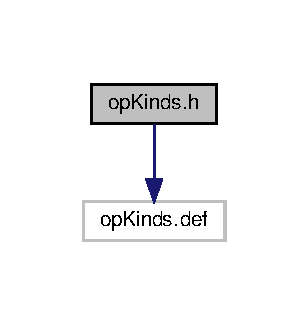
\includegraphics[width=148pt]{opKinds_8h__incl}
\end{center}
\end{figure}
This graph shows which files directly or indirectly include this file\+:\nopagebreak
\begin{figure}[H]
\begin{center}
\leavevmode
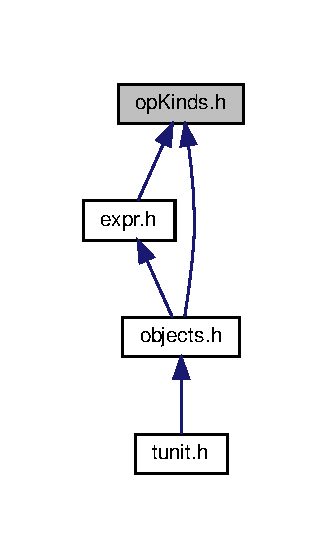
\includegraphics[width=157pt]{opKinds_8h__dep__incl}
\end{center}
\end{figure}
\subsection*{Namespaces}
\begin{DoxyCompactItemize}
\item 
 \hyperlink{namespacespan}{span}
\begin{DoxyCompactList}\small\item\em Encapsulates all of S\+P\+AN. \end{DoxyCompactList}\item 
 \hyperlink{namespacespan_1_1ir}{span\+::ir}
\begin{DoxyCompactList}\small\item\em Contains all of S\+P\+AN IR. \end{DoxyCompactList}\item 
 \hyperlink{namespacespan_1_1ir_1_1op}{span\+::ir\+::op}
\begin{DoxyCompactList}\small\item\em The operators used in expressions. \end{DoxyCompactList}\end{DoxyCompactItemize}
\subsection*{Macros}
\begin{DoxyCompactItemize}
\item 
\#define \hyperlink{opKinds_8h_aa6796f43d0f5e6dfa0eb95157e2a436f}{C\+A\+S\+T\+\_\+\+O\+P\+E\+R\+A\+T\+I\+ON}(Name)~C\+K\+\_\+\#\#Name,
\item 
\#define \hyperlink{opKinds_8h_a1958130a3b607318055053ade29ce9ea}{B\+I\+N\+A\+R\+Y\+\_\+\+O\+P\+E\+R\+A\+T\+I\+ON}(Name,  Spelling)~B\+O\+\_\+\#\#Name,
\item 
\#define \hyperlink{opKinds_8h_a22fcfba7d3c5c7952149d70bfef3ecb0}{U\+N\+A\+R\+Y\+\_\+\+O\+P\+E\+R\+A\+T\+I\+ON}(Name,  Spelling)~U\+O\+\_\+\#\#Name,
\end{DoxyCompactItemize}
\subsection*{Enumerations}
\begin{DoxyCompactItemize}
\item 
enum \hyperlink{namespacespan_1_1ir_1_1op_a04abe430db9937e27dc5df909415002b}{span\+::ir\+::op\+::\+Cast\+Kind} \begin{DoxyCompactList}\small\item\em Cast\+Kind -\/ The kind of operation required for a conversion. \end{DoxyCompactList}
\item 
enum \hyperlink{namespacespan_1_1ir_1_1op_a5741ac4595bea9e1d2821a8bb5d953e3}{span\+::ir\+::op\+::\+Binary\+Operator\+Kind} \begin{DoxyCompactList}\small\item\em All binary operators. \end{DoxyCompactList}
\item 
enum \hyperlink{namespacespan_1_1ir_1_1op_ab88ceb1213c3473d4f5fc848509dd181}{span\+::ir\+::op\+::\+Unary\+Operator\+Kind} \begin{DoxyCompactList}\small\item\em All unary operators. \end{DoxyCompactList}
\end{DoxyCompactItemize}


\subsection{Macro Definition Documentation}
\mbox{\Hypertarget{opKinds_8h_a1958130a3b607318055053ade29ce9ea}\label{opKinds_8h_a1958130a3b607318055053ade29ce9ea}} 
\index{op\+Kinds.\+h@{op\+Kinds.\+h}!B\+I\+N\+A\+R\+Y\+\_\+\+O\+P\+E\+R\+A\+T\+I\+ON@{B\+I\+N\+A\+R\+Y\+\_\+\+O\+P\+E\+R\+A\+T\+I\+ON}}
\index{B\+I\+N\+A\+R\+Y\+\_\+\+O\+P\+E\+R\+A\+T\+I\+ON@{B\+I\+N\+A\+R\+Y\+\_\+\+O\+P\+E\+R\+A\+T\+I\+ON}!op\+Kinds.\+h@{op\+Kinds.\+h}}
\subsubsection{\texorpdfstring{B\+I\+N\+A\+R\+Y\+\_\+\+O\+P\+E\+R\+A\+T\+I\+ON}{BINARY\_OPERATION}}
{\footnotesize\ttfamily \#define B\+I\+N\+A\+R\+Y\+\_\+\+O\+P\+E\+R\+A\+T\+I\+ON(\begin{DoxyParamCaption}\item[{}]{Name,  }\item[{}]{Spelling }\end{DoxyParamCaption})~B\+O\+\_\+\#\#Name,}

\mbox{\Hypertarget{opKinds_8h_aa6796f43d0f5e6dfa0eb95157e2a436f}\label{opKinds_8h_aa6796f43d0f5e6dfa0eb95157e2a436f}} 
\index{op\+Kinds.\+h@{op\+Kinds.\+h}!C\+A\+S\+T\+\_\+\+O\+P\+E\+R\+A\+T\+I\+ON@{C\+A\+S\+T\+\_\+\+O\+P\+E\+R\+A\+T\+I\+ON}}
\index{C\+A\+S\+T\+\_\+\+O\+P\+E\+R\+A\+T\+I\+ON@{C\+A\+S\+T\+\_\+\+O\+P\+E\+R\+A\+T\+I\+ON}!op\+Kinds.\+h@{op\+Kinds.\+h}}
\subsubsection{\texorpdfstring{C\+A\+S\+T\+\_\+\+O\+P\+E\+R\+A\+T\+I\+ON}{CAST\_OPERATION}}
{\footnotesize\ttfamily \#define C\+A\+S\+T\+\_\+\+O\+P\+E\+R\+A\+T\+I\+ON(\begin{DoxyParamCaption}\item[{}]{Name }\end{DoxyParamCaption})~C\+K\+\_\+\#\#Name,}

\mbox{\Hypertarget{opKinds_8h_a22fcfba7d3c5c7952149d70bfef3ecb0}\label{opKinds_8h_a22fcfba7d3c5c7952149d70bfef3ecb0}} 
\index{op\+Kinds.\+h@{op\+Kinds.\+h}!U\+N\+A\+R\+Y\+\_\+\+O\+P\+E\+R\+A\+T\+I\+ON@{U\+N\+A\+R\+Y\+\_\+\+O\+P\+E\+R\+A\+T\+I\+ON}}
\index{U\+N\+A\+R\+Y\+\_\+\+O\+P\+E\+R\+A\+T\+I\+ON@{U\+N\+A\+R\+Y\+\_\+\+O\+P\+E\+R\+A\+T\+I\+ON}!op\+Kinds.\+h@{op\+Kinds.\+h}}
\subsubsection{\texorpdfstring{U\+N\+A\+R\+Y\+\_\+\+O\+P\+E\+R\+A\+T\+I\+ON}{UNARY\_OPERATION}}
{\footnotesize\ttfamily \#define U\+N\+A\+R\+Y\+\_\+\+O\+P\+E\+R\+A\+T\+I\+ON(\begin{DoxyParamCaption}\item[{}]{Name,  }\item[{}]{Spelling }\end{DoxyParamCaption})~U\+O\+\_\+\#\#Name,}


\hypertarget{README_8md}{}\section{R\+E\+A\+D\+M\+E.\+md File Reference}
\label{README_8md}\index{R\+E\+A\+D\+M\+E.\+md@{R\+E\+A\+D\+M\+E.\+md}}

\hypertarget{tunit_8h}{}\section{tunit.\+h File Reference}
\label{tunit_8h}\index{tunit.\+h@{tunit.\+h}}
{\ttfamily \#include \char`\"{}types.\+h\char`\"{}}\newline
{\ttfamily \#include \char`\"{}objects.\+h\char`\"{}}\newline
{\ttfamily \#include $<$unordered\+\_\+map$>$}\newline
{\ttfamily \#include $<$string$>$}\newline
Include dependency graph for tunit.\+h\+:\nopagebreak
\begin{figure}[H]
\begin{center}
\leavevmode
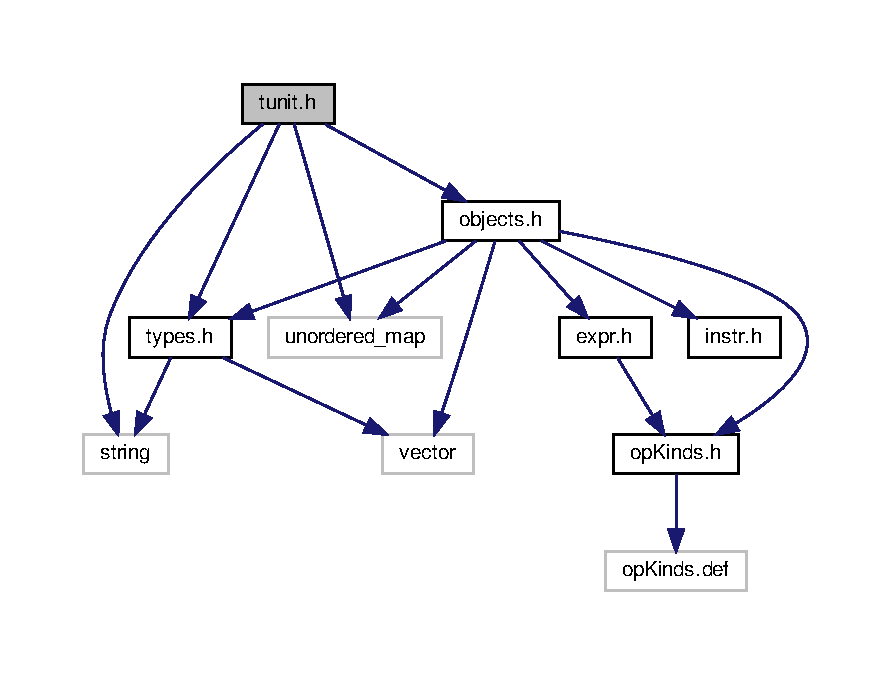
\includegraphics[width=350pt]{tunit_8h__incl}
\end{center}
\end{figure}
\subsection*{Classes}
\begin{DoxyCompactItemize}
\item 
class \hyperlink{classspan_1_1ir_1_1tunit_1_1TUnit}{span\+::ir\+::tunit\+::\+T\+Unit}
\begin{DoxyCompactList}\small\item\em Holds the complete translation unit. \end{DoxyCompactList}\end{DoxyCompactItemize}
\subsection*{Namespaces}
\begin{DoxyCompactItemize}
\item 
 \hyperlink{namespacespan}{span}
\begin{DoxyCompactList}\small\item\em Encapsulates all of S\+P\+AN. \end{DoxyCompactList}\item 
 \hyperlink{namespacespan_1_1ir}{span\+::ir}
\begin{DoxyCompactList}\small\item\em Contains all of S\+P\+AN IR. \end{DoxyCompactList}\item 
 \hyperlink{namespacespan_1_1ir_1_1tunit}{span\+::ir\+::tunit}
\end{DoxyCompactItemize}
\subsection*{Typedefs}
\begin{DoxyCompactItemize}
\item 
typedef std\+::unordered\+\_\+map$<$ \hyperlink{namespacespan_adc1e351442e4f323d37dbbb8736d003f}{span\+::\+Var\+Name}, Type $>$ \hyperlink{namespacespan_1_1ir_1_1tunit_ab87decca6ee3f2091cb24b47d831aa44}{span\+::ir\+::tunit\+::\+Var\+Map}
\begin{DoxyCompactList}\small\item\em The variables in a translation unit. \end{DoxyCompactList}\item 
typedef std\+::unordered\+\_\+map$<$ \hyperlink{namespacespan_a5184c08609df37077d47e497f83aadd1}{span\+::\+Function\+Name}, obj\+::\+Function $>$ \hyperlink{namespacespan_1_1ir_1_1tunit_a8c9ac0f8660f3f103f7b1ecb106b583b}{span\+::ir\+::tunit\+::\+Func\+Map}
\begin{DoxyCompactList}\small\item\em The functions declared/defined in a translation unit. \end{DoxyCompactList}\item 
typedef std\+::unordered\+\_\+map$<$ \hyperlink{namespacespan_a556ddaab2ad6c39fb1d89fb38182fe57}{span\+::\+Record\+Name}, types\+::\+Record $>$ \hyperlink{namespacespan_1_1ir_1_1tunit_a466edb24fa3caa23d32ca7bc2cdeac12}{span\+::ir\+::tunit\+::\+Record\+Map}
\begin{DoxyCompactList}\small\item\em The records defined in the translation unit. \end{DoxyCompactList}\end{DoxyCompactItemize}

\hypertarget{Types_8cpp}{}\section{Types.\+cpp File Reference}
\label{Types_8cpp}\index{Types.\+cpp@{Types.\+cpp}}
{\ttfamily \#include \char`\"{}types.\+h\char`\"{}}\newline
Include dependency graph for Types.\+cpp\+:\nopagebreak
\begin{figure}[H]
\begin{center}
\leavevmode
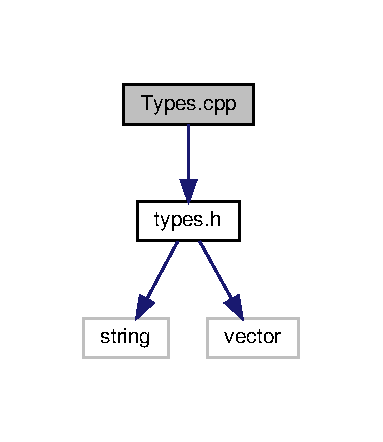
\includegraphics[width=184pt]{Types_8cpp__incl}
\end{center}
\end{figure}

\hypertarget{types_8h}{}\section{types.\+h File Reference}
\label{types_8h}\index{types.\+h@{types.\+h}}
{\ttfamily \#include $<$string$>$}\newline
{\ttfamily \#include $<$vector$>$}\newline
Include dependency graph for types.\+h\+:\nopagebreak
\begin{figure}[H]
\begin{center}
\leavevmode
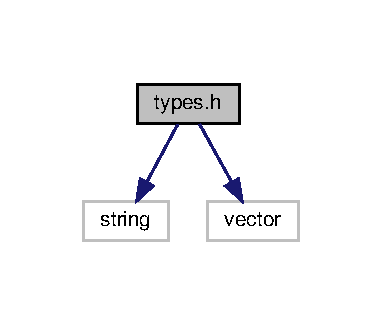
\includegraphics[width=184pt]{types_8h__incl}
\end{center}
\end{figure}
This graph shows which files directly or indirectly include this file\+:\nopagebreak
\begin{figure}[H]
\begin{center}
\leavevmode
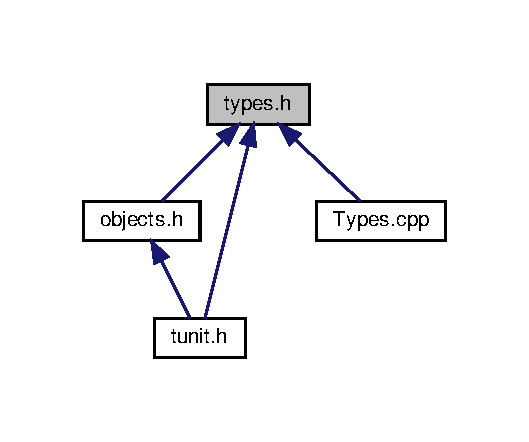
\includegraphics[width=254pt]{types_8h__dep__incl}
\end{center}
\end{figure}
\subsection*{Classes}
\begin{DoxyCompactItemize}
\item 
class \hyperlink{classspan_1_1ir_1_1types_1_1Type}{span\+::ir\+::types\+::\+Type}
\item 
class \hyperlink{classspan_1_1ir_1_1types_1_1Function}{span\+::ir\+::types\+::\+Function}
\item 
class \hyperlink{classspan_1_1ir_1_1types_1_1Record}{span\+::ir\+::types\+::\+Record}
\end{DoxyCompactItemize}
\subsection*{Namespaces}
\begin{DoxyCompactItemize}
\item 
 \hyperlink{namespacespan}{span}
\begin{DoxyCompactList}\small\item\em Encapsulates all of S\+P\+AN. \end{DoxyCompactList}\item 
 \hyperlink{namespacespan_1_1ir}{span\+::ir}
\begin{DoxyCompactList}\small\item\em Contains all of S\+P\+AN IR. \end{DoxyCompactList}\item 
 \hyperlink{namespacespan_1_1ir_1_1types}{span\+::ir\+::types}
\end{DoxyCompactItemize}
\subsection*{Macros}
\begin{DoxyCompactItemize}
\item 
\#define \hyperlink{types_8h_afdaf148a07f18d2b63f0e4a450a326f4}{B\+A\+S\+I\+C\+T\+Y\+PE}(name,  description)~T\+Y\+\_\+\#\#name,
\end{DoxyCompactItemize}
\subsection*{Typedefs}
\begin{DoxyCompactItemize}
\item 
typedef int32\+\_\+t \hyperlink{namespacespan_ab988dafbd25ab39838239b91d6a86214}{span\+::\+Basic\+Block\+Id}
\item 
typedef int32\+\_\+t \hyperlink{namespacespan_a34e8d849ca2007fe03cb1817685d08bf}{span\+::\+C\+F\+G\+Node\+Id}
\item 
typedef std\+::string \hyperlink{namespacespan_adc1e351442e4f323d37dbbb8736d003f}{span\+::\+Var\+Name}
\item 
typedef std\+::string \hyperlink{namespacespan_a5184c08609df37077d47e497f83aadd1}{span\+::\+Function\+Name}
\item 
typedef std\+::string \hyperlink{namespacespan_a556ddaab2ad6c39fb1d89fb38182fe57}{span\+::\+Record\+Name}
\end{DoxyCompactItemize}
\subsection*{Enumerations}
\begin{DoxyCompactItemize}
\item 
enum \hyperlink{namespacespan_1_1ir_1_1types_a12599995a12fb984883f13a64936de36}{span\+::ir\+::types\+::\+Basic\+Type\+Kinds} 
\end{DoxyCompactItemize}


\subsection{Macro Definition Documentation}
\mbox{\Hypertarget{types_8h_afdaf148a07f18d2b63f0e4a450a326f4}\label{types_8h_afdaf148a07f18d2b63f0e4a450a326f4}} 
\index{types.\+h@{types.\+h}!B\+A\+S\+I\+C\+T\+Y\+PE@{B\+A\+S\+I\+C\+T\+Y\+PE}}
\index{B\+A\+S\+I\+C\+T\+Y\+PE@{B\+A\+S\+I\+C\+T\+Y\+PE}!types.\+h@{types.\+h}}
\subsubsection{\texorpdfstring{B\+A\+S\+I\+C\+T\+Y\+PE}{BASICTYPE}}
{\footnotesize\ttfamily \#define B\+A\+S\+I\+C\+T\+Y\+PE(\begin{DoxyParamCaption}\item[{}]{name,  }\item[{}]{description }\end{DoxyParamCaption})~T\+Y\+\_\+\#\#name,}


%--- End generated contents ---

% Index
\backmatter
\newpage
\phantomsection
\clearemptydoublepage
\addcontentsline{toc}{chapter}{Index}
\printindex

\end{document}
